\documentclass[twoside]{book}

% Packages required by doxygen
\usepackage{fixltx2e}
\usepackage{calc}
\usepackage{doxygen}
\usepackage[export]{adjustbox} % also loads graphicx
\usepackage{graphicx}
\usepackage[utf8]{inputenc}
\usepackage{makeidx}
\usepackage{multicol}
\usepackage{multirow}
\PassOptionsToPackage{warn}{textcomp}
\usepackage{textcomp}
\usepackage[nointegrals]{wasysym}
\usepackage[table]{xcolor}

% NLS support packages
Portuguese
% Font selection
\usepackage[T1]{fontenc}
\usepackage[scaled=.90]{helvet}
\usepackage{courier}
\usepackage{amssymb}
\usepackage{sectsty}
\renewcommand{\familydefault}{\sfdefault}
\allsectionsfont{%
  \fontseries{bc}\selectfont%
  \color{darkgray}%
}
\renewcommand{\DoxyLabelFont}{%
  \fontseries{bc}\selectfont%
  \color{darkgray}%
}
\newcommand{\+}{\discretionary{\mbox{\scriptsize$\hookleftarrow$}}{}{}}

% Page & text layout
\usepackage{geometry}
\geometry{%
  a4paper,%
  top=2.5cm,%
  bottom=2.5cm,%
  left=2.5cm,%
  right=2.5cm%
}
\tolerance=750
\hfuzz=15pt
\hbadness=750
\setlength{\emergencystretch}{15pt}
\setlength{\parindent}{0cm}
\setlength{\parskip}{3ex plus 2ex minus 2ex}
\makeatletter
\renewcommand{\paragraph}{%
  \@startsection{paragraph}{4}{0ex}{-1.0ex}{1.0ex}{%
    \normalfont\normalsize\bfseries\SS@parafont%
  }%
}
\renewcommand{\subparagraph}{%
  \@startsection{subparagraph}{5}{0ex}{-1.0ex}{1.0ex}{%
    \normalfont\normalsize\bfseries\SS@subparafont%
  }%
}
\makeatother

% Headers & footers
\usepackage{fancyhdr}
\pagestyle{fancyplain}
\fancyhead[LE]{\fancyplain{}{\bfseries\thepage}}
\fancyhead[CE]{\fancyplain{}{}}
\fancyhead[RE]{\fancyplain{}{\bfseries\leftmark}}
\fancyhead[LO]{\fancyplain{}{\bfseries\rightmark}}
\fancyhead[CO]{\fancyplain{}{}}
\fancyhead[RO]{\fancyplain{}{\bfseries\thepage}}
\fancyfoot[LE]{\fancyplain{}{}}
\fancyfoot[CE]{\fancyplain{}{}}
\fancyfoot[RE]{\fancyplain{}{\bfseries\scriptsize Gerado por Doxygen }}
\fancyfoot[LO]{\fancyplain{}{\bfseries\scriptsize Gerado por Doxygen }}
\fancyfoot[CO]{\fancyplain{}{}}
\fancyfoot[RO]{\fancyplain{}{}}
\renewcommand{\footrulewidth}{0.4pt}
\renewcommand{\chaptermark}[1]{%
  \markboth{#1}{}%
}
\renewcommand{\sectionmark}[1]{%
  \markright{\thesection\ #1}%
}

% Indices & bibliography
\usepackage{natbib}
\usepackage[titles]{tocloft}
\setcounter{tocdepth}{3}
\setcounter{secnumdepth}{5}
\makeindex

% Hyperlinks (required, but should be loaded last)
\usepackage{ifpdf}
\ifpdf
  \usepackage[pdftex,pagebackref=true]{hyperref}
\else
  \usepackage[ps2pdf,pagebackref=true]{hyperref}
\fi
\hypersetup{%
  colorlinks=true,%
  linkcolor=blue,%
  citecolor=blue,%
  unicode%
}

% Custom commands
\newcommand{\clearemptydoublepage}{%
  \newpage{\pagestyle{empty}\cleardoublepage}%
}

\usepackage{caption}
\captionsetup{labelsep=space,justification=centering,font={bf},singlelinecheck=off,skip=4pt,position=top}

%===== C O N T E N T S =====

\begin{document}

% Titlepage & ToC
\hypersetup{pageanchor=false,
             bookmarksnumbered=true,
             pdfencoding=unicode
            }
\pagenumbering{roman}
\begin{titlepage}
\vspace*{7cm}
\begin{center}%
{\Large Implementing the List Abstract Data Type }\\
\vspace*{1cm}
{\large Gerado por Doxygen 1.8.11}\\
\end{center}
\end{titlepage}
\clearemptydoublepage
\tableofcontents
\clearemptydoublepage
\pagenumbering{arabic}
\hypersetup{pageanchor=true}

%--- Begin generated contents ---
\chapter{Forward List}
\label{index}\hypertarget{index}{}\begin{DoxyAuthor}{Autor}
Adelino Afonso Fernandes Avelino 

Irene Ginani Costa Pinheiro 
\end{DoxyAuthor}
\begin{DoxyDate}{Data}
May, 2016 
\end{DoxyDate}
\begin{DoxyVersion}{Versão}
1.\+0 
\end{DoxyVersion}

\chapter{Implementing the List Abstract Data Type}
\label{md_README}
\hypertarget{md_README}{}
\subsection*{Descrição}

\begin{DoxyVerb}O projeto em questão foi realizado para a disciplina de Liguagem de Programação I e visa o desenvolvimento de três classes, um vector, uma forward_list e um list (vetor, lista encadeada e lista duplamente encadeada). Para que essas classes se comportassem de forma semelhante as da biblioteca do c++ std, foi necessário desenvolver mais duas classes para cada estrutura de dado, um const_iterator e um iterator. Essas duas classes auxiliares tinham métodos de acesso a determinados pontos das estruturas de forma que se comportavam como ponteiros encapsulados.
A implementacao consiste em desenvolver funcoes basicas como: inserir elementos de diversas formas, remover elementos, modificar valores, atribuir valores, colher valores. Na implementacao tambem foi necessario o desenvolvimento de iteradores em todas as tres classes solicitadas no documento. Em virtude de facilidade de testes os drivers dos programas foram divididos em tres partes.
\end{DoxyVerb}


\subsection*{Compilação e Execucao}

\subsubsection*{Dentro de seu respectivo diretorio executar o comando referente}

$\ast$\+Vector

\$ g++ -\/std=c++11 -\/I include/ \hyperlink{drive__vector_8cpp}{src/drive\+\_\+vector.\+cpp} -\/o bin/exe \&\& ./bin/exe

$\ast$\+Forward\+\_\+list

\$ g++ -\/std=c++11 -\/I include/ \hyperlink{drive__forward__list_8cpp}{src/drive\+\_\+forward\+\_\+list.\+cpp} -\/o bin/exe \&\& ./bin/exe

$\ast$\+List

\$ g++ -\/std=c++11 -\/I include/ \hyperlink{drive_8cpp}{src/drive.\+cpp} -\/o bin/exe \&\& ./bin/exe

\subsection*{Autores\+:}


\begin{DoxyItemize}
\item Adelino Afonso Fernandes Avelino -\/ \href{mailto:adelino-afonso@hotmail.com}{\tt adelino-\/afonso@hotmail.\+com}
\item Irene Ginani Costa Pinheiro -\/ \href{mailto:ireneginani@gmail.com}{\tt ireneginani@gmail.\+com} 
\end{DoxyItemize}
\chapter{Índice da hierarquia}
\section{Hierarquia de classes}
Esta lista de heranças está organizada, dentro do possível, por ordem alfabética\+:\begin{DoxyCompactList}
\item \contentsline{section}{Forward\+\_\+list$<$ T $>$\+:\+:const\+\_\+iterator}{\pageref{class_forward__list_1_1const__iterator}}{}
\begin{DoxyCompactList}
\item \contentsline{section}{Forward\+\_\+list$<$ T $>$\+:\+:iterator}{\pageref{class_forward__list_1_1iterator}}{}
\end{DoxyCompactList}
\item \contentsline{section}{Vector$<$ Obj $>$\+:\+:const\+\_\+iterator}{\pageref{class_vector_1_1const__iterator}}{}
\begin{DoxyCompactList}
\item \contentsline{section}{Vector$<$ Obj $>$\+:\+:iterator}{\pageref{class_vector_1_1iterator}}{}
\end{DoxyCompactList}
\item \contentsline{section}{List$<$ T $>$\+:\+:const\+\_\+iterator}{\pageref{class_list_1_1const__iterator}}{}
\begin{DoxyCompactList}
\item \contentsline{section}{List$<$ T $>$\+:\+:iterator}{\pageref{class_list_1_1iterator}}{}
\end{DoxyCompactList}
\item \contentsline{section}{Forward\+\_\+list$<$ T $>$}{\pageref{class_forward__list}}{}
\item \contentsline{section}{List$<$ T $>$}{\pageref{class_list}}{}
\item \contentsline{section}{Vector$<$ Obj $>$}{\pageref{class_vector}}{}
\end{DoxyCompactList}

\chapter{Índice dos componentes}
\section{Lista de componentes}
Lista de classes, estruturas, uniões e interfaces com uma breve descrição\+:\begin{DoxyCompactList}
\item\contentsline{section}{\hyperlink{class_forward__list_1_1const__iterator}{Forward\+\_\+list$<$ T $>$\+::const\+\_\+iterator} \\*Classe \hyperlink{class_forward__list_1_1const__iterator}{const\+\_\+iterator} }{\pageref{class_forward__list_1_1const__iterator}}{}
\item\contentsline{section}{\hyperlink{class_vector_1_1const__iterator}{Vector$<$ Obj $>$\+::const\+\_\+iterator} }{\pageref{class_vector_1_1const__iterator}}{}
\item\contentsline{section}{\hyperlink{class_list_1_1const__iterator}{List$<$ T $>$\+::const\+\_\+iterator} }{\pageref{class_list_1_1const__iterator}}{}
\item\contentsline{section}{\hyperlink{class_forward__list}{Forward\+\_\+list$<$ T $>$} \\*Classe \hyperlink{class_forward__list}{Forward\+\_\+list} }{\pageref{class_forward__list}}{}
\item\contentsline{section}{\hyperlink{class_vector_1_1iterator}{Vector$<$ Obj $>$\+::iterator} }{\pageref{class_vector_1_1iterator}}{}
\item\contentsline{section}{\hyperlink{class_list_1_1iterator}{List$<$ T $>$\+::iterator} \\*Classe iterator }{\pageref{class_list_1_1iterator}}{}
\item\contentsline{section}{\hyperlink{class_forward__list_1_1iterator}{Forward\+\_\+list$<$ T $>$\+::iterator} \\*Classe iterator }{\pageref{class_forward__list_1_1iterator}}{}
\item\contentsline{section}{\hyperlink{class_list}{List$<$ T $>$} \\*Classe \hyperlink{class_list}{List} }{\pageref{class_list}}{}
\item\contentsline{section}{\hyperlink{class_vector}{Vector$<$ Obj $>$} \\*Classe \hyperlink{class_vector}{Vector} }{\pageref{class_vector}}{}
\end{DoxyCompactList}

\chapter{Índice dos ficheiros}
\section{Lista de ficheiros}
Lista de todos os ficheiros documentados com uma breve descrição\+:\begin{DoxyCompactList}
\item\contentsline{section}{Forward\+\_\+\+List/include/\hyperlink{forward__list_8h}{forward\+\_\+list.\+h} \\*Corpo da Classe \hyperlink{class_forward__list}{Forward\+\_\+list} }{\pageref{forward__list_8h}}{}
\item\contentsline{section}{Forward\+\_\+\+List/include/\hyperlink{forward__list_8inl}{forward\+\_\+list.\+inl} \\*Implementacao das funcoes da classe }{\pageref{forward__list_8inl}}{}
\item\contentsline{section}{Forward\+\_\+\+List/src/\hyperlink{drive__forward__list_8cpp}{drive\+\_\+forward\+\_\+list.\+cpp} \\*Arquivo driver }{\pageref{drive__forward__list_8cpp}}{}
\item\contentsline{section}{List/include/\hyperlink{list_8h}{list.\+h} \\*Corpo da Classe \hyperlink{class_list}{List} }{\pageref{list_8h}}{}
\item\contentsline{section}{List/include/\hyperlink{list_8inl}{list.\+inl} \\*Implementacao das funcoes da classe }{\pageref{list_8inl}}{}
\item\contentsline{section}{List/src/\hyperlink{drive_8cpp}{drive.\+cpp} \\*Arquivo driver }{\pageref{drive_8cpp}}{}
\item\contentsline{section}{V\+E\+C\+T\+O\+R/include/\hyperlink{vector_8h}{vector.\+h} \\*Corpo da Classe \hyperlink{class_vector}{Vector} }{\pageref{vector_8h}}{}
\item\contentsline{section}{V\+E\+C\+T\+O\+R/include/\hyperlink{vector_8inl}{vector.\+inl} \\*Implementacao das funcoes da classe }{\pageref{vector_8inl}}{}
\item\contentsline{section}{V\+E\+C\+T\+O\+R/src/\hyperlink{drive__vector_8cpp}{drive\+\_\+vector.\+cpp} \\*Arquivo driver }{\pageref{drive__vector_8cpp}}{}
\end{DoxyCompactList}

\chapter{Documentação da classe}
\hypertarget{class_forward__list_1_1const__iterator}{}\section{Referência à classe Forward\+\_\+list$<$ T $>$\+:\+:const\+\_\+iterator}
\label{class_forward__list_1_1const__iterator}\index{Forward\+\_\+list$<$ T $>$\+::const\+\_\+iterator@{Forward\+\_\+list$<$ T $>$\+::const\+\_\+iterator}}


Classe \hyperlink{class_forward__list_1_1const__iterator}{const\+\_\+iterator}.  




{\ttfamily \#include $<$forward\+\_\+list.\+h$>$}

Diagrama de heranças da classe Forward\+\_\+list$<$ T $>$\+:\+:const\+\_\+iterator\begin{figure}[H]
\begin{center}
\leavevmode
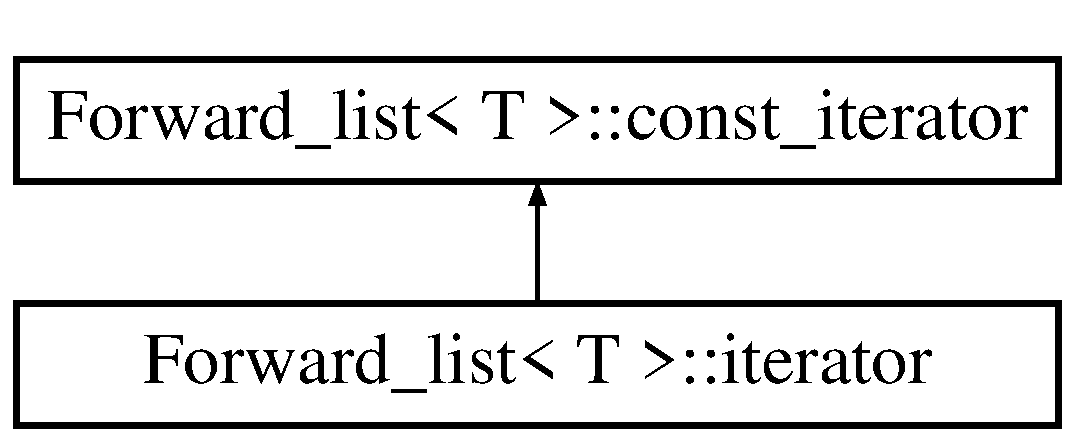
\includegraphics[height=2.000000cm]{class_forward__list_1_1const__iterator}
\end{center}
\end{figure}
\subsection*{Membros públicos}
\begin{DoxyCompactItemize}
\item 
\hyperlink{class_forward__list_1_1const__iterator_a93186c9aaa00f55fd1a83e81b177d328}{const\+\_\+iterator} ()\hypertarget{class_forward__list_1_1const__iterator_a93186c9aaa00f55fd1a83e81b177d328}{}\label{class_forward__list_1_1const__iterator_a93186c9aaa00f55fd1a83e81b177d328}

\begin{DoxyCompactList}\small\item\em Construtor padrao. \end{DoxyCompactList}\item 
const T \& \hyperlink{class_forward__list_1_1const__iterator_a06cc80474e018e57db44c6e71785d282}{operator$\ast$} () const \hypertarget{class_forward__list_1_1const__iterator_a06cc80474e018e57db44c6e71785d282}{}\label{class_forward__list_1_1const__iterator_a06cc80474e018e57db44c6e71785d282}

\begin{DoxyCompactList}\small\item\em Sobrecarga para o operador $\ast$. \end{DoxyCompactList}\item 
\hyperlink{class_forward__list_1_1const__iterator}{const\+\_\+iterator} \& \hyperlink{class_forward__list_1_1const__iterator_a5ad8f003577bf29f9405592c3ca23b4c}{operator++} ()\hypertarget{class_forward__list_1_1const__iterator_a5ad8f003577bf29f9405592c3ca23b4c}{}\label{class_forward__list_1_1const__iterator_a5ad8f003577bf29f9405592c3ca23b4c}

\begin{DoxyCompactList}\small\item\em Sobrecarga para o operador ++ (Infixo) \end{DoxyCompactList}\item 
\hyperlink{class_forward__list_1_1const__iterator}{const\+\_\+iterator} \hyperlink{class_forward__list_1_1const__iterator_ab86aea1ef2a39e5b015168a3fda9d6b3}{operator++} (int)\hypertarget{class_forward__list_1_1const__iterator_ab86aea1ef2a39e5b015168a3fda9d6b3}{}\label{class_forward__list_1_1const__iterator_ab86aea1ef2a39e5b015168a3fda9d6b3}

\begin{DoxyCompactList}\small\item\em Sobrecarga para o operador ++ (Posfixo) \end{DoxyCompactList}\item 
bool \hyperlink{class_forward__list_1_1const__iterator_aeeea7a0b0827d1771d91d477d6cdbbe1}{operator==} (const \hyperlink{class_forward__list_1_1const__iterator}{const\+\_\+iterator} \&rhs) const \hypertarget{class_forward__list_1_1const__iterator_aeeea7a0b0827d1771d91d477d6cdbbe1}{}\label{class_forward__list_1_1const__iterator_aeeea7a0b0827d1771d91d477d6cdbbe1}

\begin{DoxyCompactList}\small\item\em Sobrecarga para o operador ==. \end{DoxyCompactList}\item 
bool \hyperlink{class_forward__list_1_1const__iterator_a62c1263d95548e948bd232b41dbf3ab9}{operator!=} (const \hyperlink{class_forward__list_1_1const__iterator}{const\+\_\+iterator} \&rhs) const \hypertarget{class_forward__list_1_1const__iterator_a62c1263d95548e948bd232b41dbf3ab9}{}\label{class_forward__list_1_1const__iterator_a62c1263d95548e948bd232b41dbf3ab9}

\begin{DoxyCompactList}\small\item\em Sobrecarga para o operador !=. \end{DoxyCompactList}\end{DoxyCompactItemize}
\subsection*{Membros protegidos}
\begin{DoxyCompactItemize}
\item 
{\bfseries const\+\_\+iterator} (Node $\ast$p)\hypertarget{class_forward__list_1_1const__iterator_a4c804c58f5414d331e53ae14801fc4e3}{}\label{class_forward__list_1_1const__iterator_a4c804c58f5414d331e53ae14801fc4e3}

\end{DoxyCompactItemize}
\subsection*{Atributos Protegidos}
\begin{DoxyCompactItemize}
\item 
Node $\ast$ {\bfseries current}\hypertarget{class_forward__list_1_1const__iterator_a78f2dc73c3162a872fe473639ff9727e}{}\label{class_forward__list_1_1const__iterator_a78f2dc73c3162a872fe473639ff9727e}

\end{DoxyCompactItemize}
\subsection*{Amigos}
\begin{DoxyCompactItemize}
\item 
class {\bfseries Forward\+\_\+list$<$ T $>$}\hypertarget{class_forward__list_1_1const__iterator_a3248a6782762842dd0d50fa2ff16e968}{}\label{class_forward__list_1_1const__iterator_a3248a6782762842dd0d50fa2ff16e968}

\end{DoxyCompactItemize}


\subsection{Descrição detalhada}
\subsubsection*{template$<$typename T$>$\\*
class Forward\+\_\+list$<$ T $>$\+::const\+\_\+iterator}

Classe \hyperlink{class_forward__list_1_1const__iterator}{const\+\_\+iterator}. 

A documentação para esta classe foi gerada a partir do seguinte ficheiro\+:\begin{DoxyCompactItemize}
\item 
Forward\+\_\+\+List/include/\hyperlink{forward__list_8h}{forward\+\_\+list.\+h}\end{DoxyCompactItemize}

\hypertarget{class_vector_1_1const__iterator}{}\section{Referência à classe Vector$<$ Obj $>$\+:\+:const\+\_\+iterator}
\label{class_vector_1_1const__iterator}\index{Vector$<$ Obj $>$\+::const\+\_\+iterator@{Vector$<$ Obj $>$\+::const\+\_\+iterator}}
Diagrama de heranças da classe Vector$<$ Obj $>$\+:\+:const\+\_\+iterator\begin{figure}[H]
\begin{center}
\leavevmode
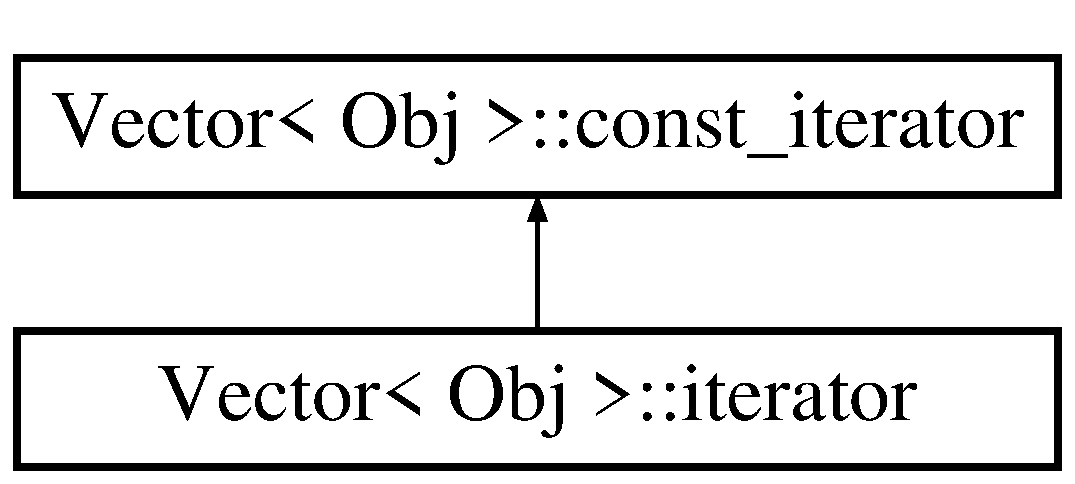
\includegraphics[height=2.000000cm]{class_vector_1_1const__iterator}
\end{center}
\end{figure}
\subsection*{Membros públicos}
\begin{DoxyCompactItemize}
\item 
\hyperlink{class_vector_1_1const__iterator_af954f0523c7ba74f7c88f86710df4cc6}{const\+\_\+iterator} ()\hypertarget{class_vector_1_1const__iterator_af954f0523c7ba74f7c88f86710df4cc6}{}\label{class_vector_1_1const__iterator_af954f0523c7ba74f7c88f86710df4cc6}

\begin{DoxyCompactList}\small\item\em Construtor padrao. \end{DoxyCompactList}\item 
const Obj \& \hyperlink{class_vector_1_1const__iterator_a33dc4eac4d02f61a73c3b456400064a1}{operator$\ast$} () const \hypertarget{class_vector_1_1const__iterator_a33dc4eac4d02f61a73c3b456400064a1}{}\label{class_vector_1_1const__iterator_a33dc4eac4d02f61a73c3b456400064a1}

\begin{DoxyCompactList}\small\item\em Sobrecarga para o operador $\ast$. \end{DoxyCompactList}\item 
\hyperlink{class_vector_1_1const__iterator}{const\+\_\+iterator} \& \hyperlink{class_vector_1_1const__iterator_adf1541d788766e7e857371642342bd54}{operator++} ()\hypertarget{class_vector_1_1const__iterator_adf1541d788766e7e857371642342bd54}{}\label{class_vector_1_1const__iterator_adf1541d788766e7e857371642342bd54}

\begin{DoxyCompactList}\small\item\em Sobrecarga para o operador ++ (Infixo) \end{DoxyCompactList}\item 
\hyperlink{class_vector_1_1const__iterator}{const\+\_\+iterator} \hyperlink{class_vector_1_1const__iterator_a598c3874b5f64f401650bcf108a6d953}{operator++} (int)\hypertarget{class_vector_1_1const__iterator_a598c3874b5f64f401650bcf108a6d953}{}\label{class_vector_1_1const__iterator_a598c3874b5f64f401650bcf108a6d953}

\begin{DoxyCompactList}\small\item\em Sobrecarga para o operador ++ (Posfixo) \end{DoxyCompactList}\item 
bool \hyperlink{class_vector_1_1const__iterator_a1eeb6debc8a581acb7a88d66ced8914c}{operator==} (const \hyperlink{class_vector_1_1const__iterator}{const\+\_\+iterator} \&rhs) const \hypertarget{class_vector_1_1const__iterator_a1eeb6debc8a581acb7a88d66ced8914c}{}\label{class_vector_1_1const__iterator_a1eeb6debc8a581acb7a88d66ced8914c}

\begin{DoxyCompactList}\small\item\em Sobrecarga para o operador ==. \end{DoxyCompactList}\item 
bool \hyperlink{class_vector_1_1const__iterator_a0e3161e20da4a0971a09dd294057e72a}{operator!=} (const \hyperlink{class_vector_1_1const__iterator}{const\+\_\+iterator} \&rhs) const \hypertarget{class_vector_1_1const__iterator_a0e3161e20da4a0971a09dd294057e72a}{}\label{class_vector_1_1const__iterator_a0e3161e20da4a0971a09dd294057e72a}

\begin{DoxyCompactList}\small\item\em Sobrecarga para o operador !=. \end{DoxyCompactList}\end{DoxyCompactItemize}
\subsection*{Membros protegidos}
\begin{DoxyCompactItemize}
\item 
{\bfseries const\+\_\+iterator} (Obj $\ast$x)\hypertarget{class_vector_1_1const__iterator_ab7a8718b0a35ab2e8e6c2c669db50672}{}\label{class_vector_1_1const__iterator_ab7a8718b0a35ab2e8e6c2c669db50672}

\end{DoxyCompactItemize}
\subsection*{Atributos Protegidos}
\begin{DoxyCompactItemize}
\item 
Obj $\ast$ {\bfseries current}\hypertarget{class_vector_1_1const__iterator_ac3f8518218a27c6a0aff658955b80079}{}\label{class_vector_1_1const__iterator_ac3f8518218a27c6a0aff658955b80079}

\end{DoxyCompactItemize}
\subsection*{Amigos}
\begin{DoxyCompactItemize}
\item 
class {\bfseries Vector$<$ Obj $>$}\hypertarget{class_vector_1_1const__iterator_a93580d986919dca737b45fdf1c366bfa}{}\label{class_vector_1_1const__iterator_a93580d986919dca737b45fdf1c366bfa}

\end{DoxyCompactItemize}


A documentação para esta classe foi gerada a partir do seguinte ficheiro\+:\begin{DoxyCompactItemize}
\item 
V\+E\+C\+T\+O\+R/include/\hyperlink{vector_8h}{vector.\+h}\end{DoxyCompactItemize}

\hypertarget{class_list_1_1const__iterator}{}\section{Referência à classe List$<$ T $>$\+:\+:const\+\_\+iterator}
\label{class_list_1_1const__iterator}\index{List$<$ T $>$\+::const\+\_\+iterator@{List$<$ T $>$\+::const\+\_\+iterator}}
Diagrama de heranças da classe List$<$ T $>$\+:\+:const\+\_\+iterator\begin{figure}[H]
\begin{center}
\leavevmode
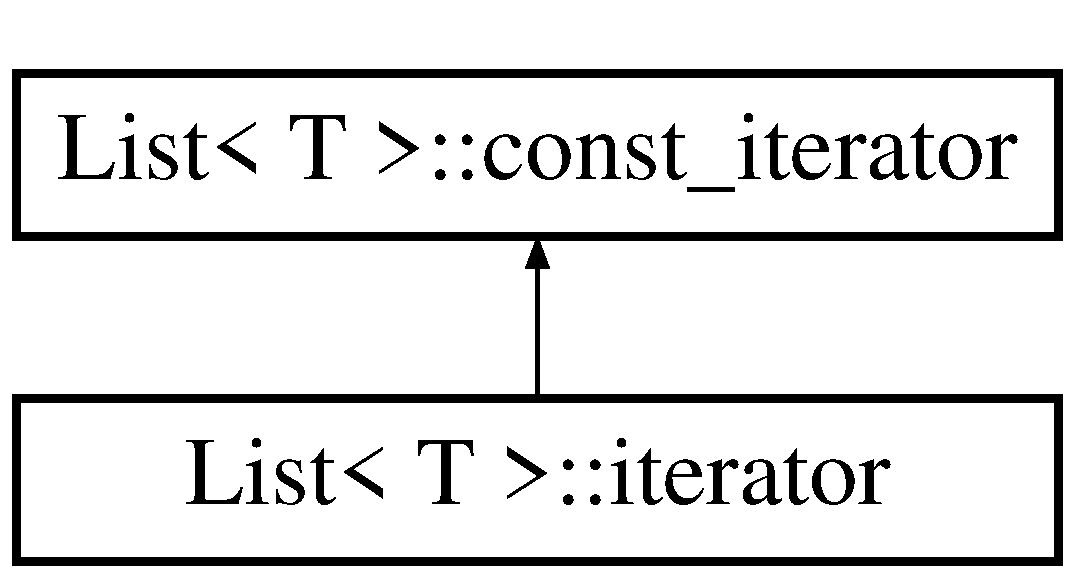
\includegraphics[height=2.000000cm]{class_list_1_1const__iterator}
\end{center}
\end{figure}
\subsection*{Membros públicos}
\begin{DoxyCompactItemize}
\item 
\hyperlink{class_list_1_1const__iterator_a504c0d1347b6fc165a41176065852e35}{const\+\_\+iterator} ()\hypertarget{class_list_1_1const__iterator_a504c0d1347b6fc165a41176065852e35}{}\label{class_list_1_1const__iterator_a504c0d1347b6fc165a41176065852e35}

\begin{DoxyCompactList}\small\item\em Construtor padrao. \end{DoxyCompactList}\item 
const T \& \hyperlink{class_list_1_1const__iterator_a6d061aa3f906a651f9c3c5a18e17c4e1}{operator$\ast$} () const \hypertarget{class_list_1_1const__iterator_a6d061aa3f906a651f9c3c5a18e17c4e1}{}\label{class_list_1_1const__iterator_a6d061aa3f906a651f9c3c5a18e17c4e1}

\begin{DoxyCompactList}\small\item\em Sobrecarga para o operador $\ast$. \end{DoxyCompactList}\item 
\hyperlink{class_list_1_1const__iterator}{const\+\_\+iterator} \& \hyperlink{class_list_1_1const__iterator_a56734329e70fcd03620d3259fee42cce}{operator++} ()\hypertarget{class_list_1_1const__iterator_a56734329e70fcd03620d3259fee42cce}{}\label{class_list_1_1const__iterator_a56734329e70fcd03620d3259fee42cce}

\begin{DoxyCompactList}\small\item\em Sobrecarga para o operador ++ (Infixo) \end{DoxyCompactList}\item 
\hyperlink{class_list_1_1const__iterator}{const\+\_\+iterator} \hyperlink{class_list_1_1const__iterator_ad33d9fb3bcbc5e460459317f04c28a78}{operator++} (int)\hypertarget{class_list_1_1const__iterator_ad33d9fb3bcbc5e460459317f04c28a78}{}\label{class_list_1_1const__iterator_ad33d9fb3bcbc5e460459317f04c28a78}

\begin{DoxyCompactList}\small\item\em Sobrecarga para o operador ++ (Posfixo) \end{DoxyCompactList}\item 
\hyperlink{class_list_1_1const__iterator}{const\+\_\+iterator} \& {\bfseries operator-\/-\/} ()\hypertarget{class_list_1_1const__iterator_aeccf9baf7498dafa7223225ee7aeaaf1}{}\label{class_list_1_1const__iterator_aeccf9baf7498dafa7223225ee7aeaaf1}

\item 
\hyperlink{class_list_1_1const__iterator}{const\+\_\+iterator} \hyperlink{class_list_1_1const__iterator_afc371e17d95507b573e9979767b9143d}{operator-\/-\/} (int)\hypertarget{class_list_1_1const__iterator_afc371e17d95507b573e9979767b9143d}{}\label{class_list_1_1const__iterator_afc371e17d95507b573e9979767b9143d}

\begin{DoxyCompactList}\small\item\em Sobrecarga para o operador ++ (Posfixo) \end{DoxyCompactList}\item 
bool \hyperlink{class_list_1_1const__iterator_ae8b8108b73e0cd8ea487d3d9c7d31e3b}{operator==} (const \hyperlink{class_list_1_1const__iterator}{const\+\_\+iterator} \&rhs) const \hypertarget{class_list_1_1const__iterator_ae8b8108b73e0cd8ea487d3d9c7d31e3b}{}\label{class_list_1_1const__iterator_ae8b8108b73e0cd8ea487d3d9c7d31e3b}

\begin{DoxyCompactList}\small\item\em Sobrecarga para o operador ==. \end{DoxyCompactList}\item 
bool \hyperlink{class_list_1_1const__iterator_af82ef9c2663c8cbe58404ac9c4c86bd3}{operator!=} (const \hyperlink{class_list_1_1const__iterator}{const\+\_\+iterator} \&rhs) const \hypertarget{class_list_1_1const__iterator_af82ef9c2663c8cbe58404ac9c4c86bd3}{}\label{class_list_1_1const__iterator_af82ef9c2663c8cbe58404ac9c4c86bd3}

\begin{DoxyCompactList}\small\item\em Sobrecarga para o operador !=. \end{DoxyCompactList}\end{DoxyCompactItemize}
\subsection*{Membros protegidos}
\begin{DoxyCompactItemize}
\item 
{\bfseries const\+\_\+iterator} (Node $\ast$p)\hypertarget{class_list_1_1const__iterator_a1dac9ee8bac44d9a4099b713fb8a1507}{}\label{class_list_1_1const__iterator_a1dac9ee8bac44d9a4099b713fb8a1507}

\end{DoxyCompactItemize}
\subsection*{Atributos Protegidos}
\begin{DoxyCompactItemize}
\item 
Node $\ast$ {\bfseries current}\hypertarget{class_list_1_1const__iterator_a8770ec36dd21c04484aa7918734d8e00}{}\label{class_list_1_1const__iterator_a8770ec36dd21c04484aa7918734d8e00}

\end{DoxyCompactItemize}
\subsection*{Amigos}
\begin{DoxyCompactItemize}
\item 
class {\bfseries List$<$ T $>$}\hypertarget{class_list_1_1const__iterator_adfa51a0eca1eba953f68ca3f65cdaa05}{}\label{class_list_1_1const__iterator_adfa51a0eca1eba953f68ca3f65cdaa05}

\end{DoxyCompactItemize}


A documentação para esta classe foi gerada a partir do seguinte ficheiro\+:\begin{DoxyCompactItemize}
\item 
List/include/\hyperlink{list_8h}{list.\+h}\end{DoxyCompactItemize}

\hypertarget{class_forward__list}{}\section{Referência à classe Template Forward\+\_\+list$<$ T $>$}
\label{class_forward__list}\index{Forward\+\_\+list$<$ T $>$@{Forward\+\_\+list$<$ T $>$}}


Classe \hyperlink{class_forward__list}{Forward\+\_\+list}.  




{\ttfamily \#include $<$forward\+\_\+list.\+h$>$}

\subsection*{Componentes}
\begin{DoxyCompactItemize}
\item 
class \hyperlink{class_forward__list_1_1const__iterator}{const\+\_\+iterator}
\begin{DoxyCompactList}\small\item\em Classe \hyperlink{class_forward__list_1_1const__iterator}{const\+\_\+iterator}. \end{DoxyCompactList}\item 
class \hyperlink{class_forward__list_1_1iterator}{iterator}
\begin{DoxyCompactList}\small\item\em Classe iterator. \end{DoxyCompactList}\end{DoxyCompactItemize}
\subsection*{Membros públicos}
\begin{DoxyCompactItemize}
\item 
\hyperlink{class_forward__list_aff553d52bc9688edecf161d1d2c0ac16}{Forward\+\_\+list} ()\hypertarget{class_forward__list_aff553d52bc9688edecf161d1d2c0ac16}{}\label{class_forward__list_aff553d52bc9688edecf161d1d2c0ac16}

\begin{DoxyCompactList}\small\item\em Construtor padrão da classe \hyperlink{class_forward__list}{Forward\+\_\+list} Seta os valores alocando novos nós. \end{DoxyCompactList}\item 
\hyperlink{class_forward__list_a05d2a10cf24da5f4c747a4775ad8841f}{$\sim$\+Forward\+\_\+list} ()\hypertarget{class_forward__list_a05d2a10cf24da5f4c747a4775ad8841f}{}\label{class_forward__list_a05d2a10cf24da5f4c747a4775ad8841f}

\begin{DoxyCompactList}\small\item\em Destrutor da classe \hyperlink{class_forward__list}{Forward\+\_\+list} Destroi o m\+\_\+head e o m\+\_\+tail. \end{DoxyCompactList}\item 
\hyperlink{class_forward__list_a5390537baf247165b6a74ef44802ceac}{Forward\+\_\+list} (const \hyperlink{class_forward__list}{Forward\+\_\+list} \&list)\hypertarget{class_forward__list_a5390537baf247165b6a74ef44802ceac}{}\label{class_forward__list_a5390537baf247165b6a74ef44802ceac}

\begin{DoxyCompactList}\small\item\em Construtor cópia da classe \hyperlink{class_forward__list}{Forward\+\_\+list} Faz uma cópia de todos os valores do objeto no qual se quer copiar. \end{DoxyCompactList}\item 
\hyperlink{class_forward__list_a6c812f45a8e1e8e6d591c138042f1fd8}{Forward\+\_\+list} (\hyperlink{class_forward__list}{Forward\+\_\+list} \&\&list)\hypertarget{class_forward__list_a6c812f45a8e1e8e6d591c138042f1fd8}{}\label{class_forward__list_a6c812f45a8e1e8e6d591c138042f1fd8}

\begin{DoxyCompactList}\small\item\em Construtor move da classe \hyperlink{class_forward__list}{Forward\+\_\+list} Move todos os elementos de um objeto de uma classe para outro objeto. \end{DoxyCompactList}\item 
\hyperlink{class_forward__list}{Forward\+\_\+list} \& \hyperlink{class_forward__list_a3220cc90bc1bb27b0e619c337fab15d1}{operator=} (const \hyperlink{class_forward__list}{Forward\+\_\+list} \&list)
\begin{DoxyCompactList}\small\item\em Sobrecarga do operador cópia   $\ast$ @ Param list O elemento a ser copiado   $\ast$. \end{DoxyCompactList}\item 
\hyperlink{class_forward__list}{Forward\+\_\+list} \& \hyperlink{class_forward__list_a00a7638bfa3b628a8593a5860c94aea2}{operator=} (\hyperlink{class_forward__list}{Forward\+\_\+list} \&\&list)
\begin{DoxyCompactList}\small\item\em Sobrecarga do operador move   $\ast$ @ Param list O elemento a ser movido   $\ast$. \end{DoxyCompactList}\item 
\hyperlink{class_forward__list_1_1iterator}{iterator} \hyperlink{class_forward__list_a07be2a83d44326a8cd0b5cdf1f812bd4}{before\+\_\+begin} ()
\begin{DoxyCompactList}\small\item\em Pega um iterador apontando para o inicio da lista. \end{DoxyCompactList}\item 
\hyperlink{class_forward__list_1_1iterator}{iterator} \hyperlink{class_forward__list_a6bb9ba980c3609dddf08078b6d58f817}{begin} ()
\begin{DoxyCompactList}\small\item\em Pega um iterador apontando para o primeiro elemento da lista. \end{DoxyCompactList}\item 
\hyperlink{class_forward__list_1_1iterator}{iterator} \hyperlink{class_forward__list_a468b0e5cf01c8fc2750e0e5f960a76a3}{end} ()
\begin{DoxyCompactList}\small\item\em Pega um iterador apontando para o ultimo elemento da lista. \end{DoxyCompactList}\item 
\hyperlink{class_forward__list_1_1const__iterator}{const\+\_\+iterator} \hyperlink{class_forward__list_af4521653f814b65d2d6553e10d68b004}{cbefore\+\_\+begin} () const 
\begin{DoxyCompactList}\small\item\em Pega um iterador apontando para o inicio da lista. \end{DoxyCompactList}\item 
\hyperlink{class_forward__list_1_1const__iterator}{const\+\_\+iterator} \hyperlink{class_forward__list_a9e4499538c8d69d746e7d09c085a6ced}{cbegin} () const 
\begin{DoxyCompactList}\small\item\em Pega um iterador const apontando para o primeiro elemento da lista. \end{DoxyCompactList}\item 
\hyperlink{class_forward__list_1_1const__iterator}{const\+\_\+iterator} \hyperlink{class_forward__list_aad341f8fad1e7aafb207434d8818f82a}{cend} () const 
\begin{DoxyCompactList}\small\item\em Pega um iterador const apontando para o ultimo elemento da lista. \end{DoxyCompactList}\item 
int \hyperlink{class_forward__list_a0773c719de2e80aa3185c85a42beea3b}{size} () const 
\begin{DoxyCompactList}\small\item\em Colhe o tamanho da lista. \end{DoxyCompactList}\item 
bool \hyperlink{class_forward__list_a765dc4c49b06c6debf4f34921e764a1f}{empty} () const 
\begin{DoxyCompactList}\small\item\em Verifica se a lista está vazia. \end{DoxyCompactList}\item 
void \hyperlink{class_forward__list_a7416894cdbf5076501c1008e65415a7e}{clear} ()
\begin{DoxyCompactList}\small\item\em Deleta todos os elementos da lista. \end{DoxyCompactList}\item 
T \& \hyperlink{class_forward__list_ade0b98cfad0e480195fb809f2e489409}{front} ()
\begin{DoxyCompactList}\small\item\em Pega o elemento da frente da lista. \end{DoxyCompactList}\item 
const T \& \hyperlink{class_forward__list_a5bfa5ba82db8a60b3477e36e1455baa2}{front} () const 
\begin{DoxyCompactList}\small\item\em Pega o elemento da frente da lista. \end{DoxyCompactList}\item 
T \& \hyperlink{class_forward__list_acd6cd5c5bf33df552796be306ccdf11c}{back} ()
\begin{DoxyCompactList}\small\item\em Pega o elemento do final da lista. \end{DoxyCompactList}\item 
const T \& \hyperlink{class_forward__list_ad38f7c3c99bd5cd5726e060c81687828}{back} () const 
\begin{DoxyCompactList}\small\item\em Pega o elemento do final da lista. \end{DoxyCompactList}\item 
void \hyperlink{class_forward__list_a0774f069e39bc80136d2c78e77b75aee}{push\+\_\+front} (const T \&x)
\begin{DoxyCompactList}\small\item\em Insere Elementos na frente da lista. \end{DoxyCompactList}\item 
void \hyperlink{class_forward__list_a51faf6177fe22a6762362bdeda69c5c8}{push\+\_\+back} (const T \&x)
\begin{DoxyCompactList}\small\item\em Insere Elementos no final da lista. \end{DoxyCompactList}\item 
void \hyperlink{class_forward__list_a7abff5d3df864ba0a82da91bff676261}{pop\+\_\+front} ()
\begin{DoxyCompactList}\small\item\em Deleta Elementos na frente da lista. \end{DoxyCompactList}\item 
void \hyperlink{class_forward__list_a503678bac3a83b4cb48ba4628c11c8a7}{pop\+\_\+back} ()
\begin{DoxyCompactList}\small\item\em Deleta Elementos no final da lista. \end{DoxyCompactList}\item 
void \hyperlink{class_forward__list_ace9a774c6f8ec3cd2b79b61a25b372f2}{assign} (const T \&value)
\begin{DoxyCompactList}\small\item\em Insere o elemento em todas as posicoes da lista. \end{DoxyCompactList}\item 
void \hyperlink{class_forward__list_a53efa28f4498425a08b2ef2f63bd9907}{assign} (std\+::initializer\+\_\+list$<$ T $>$ ilist)
\begin{DoxyCompactList}\small\item\em Insere o elemento do tipo initializer\+\_\+list. \end{DoxyCompactList}\item 
\hyperlink{class_forward__list_1_1iterator}{iterator} \hyperlink{class_forward__list_a5514b9b2cd9bd335e427a5723a4f1e4c}{insert\+\_\+after} (\hyperlink{class_forward__list_1_1const__iterator}{const\+\_\+iterator} itr, const T \&x)
\begin{DoxyCompactList}\small\item\em Insere um elemento em uma posicao passada por parametro. \end{DoxyCompactList}\item 
\hyperlink{class_forward__list_1_1iterator}{iterator} \hyperlink{class_forward__list_af509938caeb03b51e3308a506fc4b66f}{insert\+\_\+after} (\hyperlink{class_forward__list_1_1const__iterator}{const\+\_\+iterator} pos, std\+::initializer\+\_\+list$<$ T $>$ ilist)
\begin{DoxyCompactList}\small\item\em Insere uma lista na lista iterador passada por parametro. \end{DoxyCompactList}\item 
\hyperlink{class_forward__list_1_1iterator}{iterator} \hyperlink{class_forward__list_ae9fd9be0427275ec96a138fe88d9bbce}{erase\+\_\+after} (\hyperlink{class_forward__list_1_1const__iterator}{const\+\_\+iterator} itr)
\begin{DoxyCompactList}\small\item\em Apaga um elemento em uma posicao passada por parametro. \end{DoxyCompactList}\item 
\hyperlink{class_forward__list_1_1iterator}{iterator} \hyperlink{class_forward__list_ac995fdf90fbd2a22976ba8cede63d3f7}{erase\+\_\+after} (\hyperlink{class_forward__list_1_1const__iterator}{const\+\_\+iterator} first, \hyperlink{class_forward__list_1_1const__iterator}{const\+\_\+iterator} last)
\begin{DoxyCompactList}\small\item\em Apaga os elementos em um intervalo passado por parametro. \end{DoxyCompactList}\item 
\hyperlink{class_forward__list_1_1const__iterator}{const\+\_\+iterator} \hyperlink{class_forward__list_a206b61948c4df18b4ab32071bbc1829c}{find} (const T \&x) const 
\begin{DoxyCompactList}\small\item\em Procura um elemento na lista. \end{DoxyCompactList}\end{DoxyCompactItemize}


\subsection{Descrição detalhada}
\subsubsection*{template$<$typename T$>$\\*
class Forward\+\_\+list$<$ T $>$}

Classe \hyperlink{class_forward__list}{Forward\+\_\+list}. 

Assinaturas das funções e definição da classe \hyperlink{class_forward__list}{Forward\+\_\+list} 

\subsection{Documentação dos métodos}
\index{Forward\+\_\+list@{Forward\+\_\+list}!assign@{assign}}
\index{assign@{assign}!Forward\+\_\+list@{Forward\+\_\+list}}
\subsubsection[{\texorpdfstring{assign(const T \&value)}{assign(const T &value)}}]{\setlength{\rightskip}{0pt plus 5cm}template$<$typename T $>$ void {\bf Forward\+\_\+list}$<$ T $>$\+::assign (
\begin{DoxyParamCaption}
\item[{const T \&}]{value}
\end{DoxyParamCaption}
)}\hypertarget{class_forward__list_ace9a774c6f8ec3cd2b79b61a25b372f2}{}\label{class_forward__list_ace9a774c6f8ec3cd2b79b61a25b372f2}


Insere o elemento em todas as posicoes da lista. 


\begin{DoxyParams}{Parâmetros}
{\em value} & Elemento a ser inserido \\
\hline
\end{DoxyParams}
\begin{DoxyReturn}{Retorna}
void 
\end{DoxyReturn}
\index{Forward\+\_\+list@{Forward\+\_\+list}!assign@{assign}}
\index{assign@{assign}!Forward\+\_\+list@{Forward\+\_\+list}}
\subsubsection[{\texorpdfstring{assign(std\+::initializer\+\_\+list$<$ T $>$ ilist)}{assign(std::initializer_list< T > ilist)}}]{\setlength{\rightskip}{0pt plus 5cm}template$<$typename T $>$ void {\bf Forward\+\_\+list}$<$ T $>$\+::assign (
\begin{DoxyParamCaption}
\item[{std\+::initializer\+\_\+list$<$ T $>$}]{ilist}
\end{DoxyParamCaption}
)}\hypertarget{class_forward__list_a53efa28f4498425a08b2ef2f63bd9907}{}\label{class_forward__list_a53efa28f4498425a08b2ef2f63bd9907}


Insere o elemento do tipo initializer\+\_\+list. 


\begin{DoxyParams}{Parâmetros}
{\em ilist} & Lista a ser inserida \\
\hline
\end{DoxyParams}
\begin{DoxyReturn}{Retorna}
void 
\end{DoxyReturn}
\index{Forward\+\_\+list@{Forward\+\_\+list}!back@{back}}
\index{back@{back}!Forward\+\_\+list@{Forward\+\_\+list}}
\subsubsection[{\texorpdfstring{back()}{back()}}]{\setlength{\rightskip}{0pt plus 5cm}template$<$typename T $>$ T \& {\bf Forward\+\_\+list}$<$ T $>$\+::back (
\begin{DoxyParamCaption}
{}
\end{DoxyParamCaption}
)}\hypertarget{class_forward__list_acd6cd5c5bf33df552796be306ccdf11c}{}\label{class_forward__list_acd6cd5c5bf33df552796be306ccdf11c}


Pega o elemento do final da lista. 

\begin{DoxyReturn}{Retorna}
A referência para o ultimo elemento 
\end{DoxyReturn}
\index{Forward\+\_\+list@{Forward\+\_\+list}!back@{back}}
\index{back@{back}!Forward\+\_\+list@{Forward\+\_\+list}}
\subsubsection[{\texorpdfstring{back() const }{back() const }}]{\setlength{\rightskip}{0pt plus 5cm}template$<$typename T $>$ const T \& {\bf Forward\+\_\+list}$<$ T $>$\+::back (
\begin{DoxyParamCaption}
{}
\end{DoxyParamCaption}
) const}\hypertarget{class_forward__list_ad38f7c3c99bd5cd5726e060c81687828}{}\label{class_forward__list_ad38f7c3c99bd5cd5726e060c81687828}


Pega o elemento do final da lista. 

\begin{DoxyReturn}{Retorna}
A referência const para o ultimo elemento 
\end{DoxyReturn}
\index{Forward\+\_\+list@{Forward\+\_\+list}!before\+\_\+begin@{before\+\_\+begin}}
\index{before\+\_\+begin@{before\+\_\+begin}!Forward\+\_\+list@{Forward\+\_\+list}}
\subsubsection[{\texorpdfstring{before\+\_\+begin()}{before_begin()}}]{\setlength{\rightskip}{0pt plus 5cm}template$<$typename T $>$ {\bf Forward\+\_\+list}$<$ T $>$\+::{\bf iterator} {\bf Forward\+\_\+list}$<$ T $>$\+::before\+\_\+begin (
\begin{DoxyParamCaption}
{}
\end{DoxyParamCaption}
)}\hypertarget{class_forward__list_a07be2a83d44326a8cd0b5cdf1f812bd4}{}\label{class_forward__list_a07be2a83d44326a8cd0b5cdf1f812bd4}


Pega um iterador apontando para o inicio da lista. 

  $\ast$ \begin{DoxyReturn}{Retorna}
Um iterador para o inicio da lista 
\end{DoxyReturn}
\index{Forward\+\_\+list@{Forward\+\_\+list}!begin@{begin}}
\index{begin@{begin}!Forward\+\_\+list@{Forward\+\_\+list}}
\subsubsection[{\texorpdfstring{begin()}{begin()}}]{\setlength{\rightskip}{0pt plus 5cm}template$<$typename T $>$ {\bf Forward\+\_\+list}$<$ T $>$\+::{\bf iterator} {\bf Forward\+\_\+list}$<$ T $>$\+::begin (
\begin{DoxyParamCaption}
{}
\end{DoxyParamCaption}
)}\hypertarget{class_forward__list_a6bb9ba980c3609dddf08078b6d58f817}{}\label{class_forward__list_a6bb9ba980c3609dddf08078b6d58f817}


Pega um iterador apontando para o primeiro elemento da lista. 

  $\ast$ \begin{DoxyReturn}{Retorna}
Um iterador apontando para o primeiro elemento da lista 
\end{DoxyReturn}
\index{Forward\+\_\+list@{Forward\+\_\+list}!cbefore\+\_\+begin@{cbefore\+\_\+begin}}
\index{cbefore\+\_\+begin@{cbefore\+\_\+begin}!Forward\+\_\+list@{Forward\+\_\+list}}
\subsubsection[{\texorpdfstring{cbefore\+\_\+begin() const }{cbefore_begin() const }}]{\setlength{\rightskip}{0pt plus 5cm}template$<$typename T $>$ {\bf Forward\+\_\+list}$<$ T $>$\+::{\bf const\+\_\+iterator} {\bf Forward\+\_\+list}$<$ T $>$\+::cbefore\+\_\+begin (
\begin{DoxyParamCaption}
{}
\end{DoxyParamCaption}
) const}\hypertarget{class_forward__list_af4521653f814b65d2d6553e10d68b004}{}\label{class_forward__list_af4521653f814b65d2d6553e10d68b004}


Pega um iterador apontando para o inicio da lista. 

  $\ast$ \begin{DoxyReturn}{Retorna}
Um iterador para o inicio da lista 
\end{DoxyReturn}
\index{Forward\+\_\+list@{Forward\+\_\+list}!cbegin@{cbegin}}
\index{cbegin@{cbegin}!Forward\+\_\+list@{Forward\+\_\+list}}
\subsubsection[{\texorpdfstring{cbegin() const }{cbegin() const }}]{\setlength{\rightskip}{0pt plus 5cm}template$<$typename T $>$ {\bf Forward\+\_\+list}$<$ T $>$\+::{\bf const\+\_\+iterator} {\bf Forward\+\_\+list}$<$ T $>$\+::cbegin (
\begin{DoxyParamCaption}
{}
\end{DoxyParamCaption}
) const}\hypertarget{class_forward__list_a9e4499538c8d69d746e7d09c085a6ced}{}\label{class_forward__list_a9e4499538c8d69d746e7d09c085a6ced}


Pega um iterador const apontando para o primeiro elemento da lista. 

  $\ast$ \begin{DoxyReturn}{Retorna}
Um iterador apontando para o primeiro elemento da lista 
\end{DoxyReturn}
\index{Forward\+\_\+list@{Forward\+\_\+list}!cend@{cend}}
\index{cend@{cend}!Forward\+\_\+list@{Forward\+\_\+list}}
\subsubsection[{\texorpdfstring{cend() const }{cend() const }}]{\setlength{\rightskip}{0pt plus 5cm}template$<$typename T $>$ {\bf Forward\+\_\+list}$<$ T $>$\+::{\bf const\+\_\+iterator} {\bf Forward\+\_\+list}$<$ T $>$\+::cend (
\begin{DoxyParamCaption}
{}
\end{DoxyParamCaption}
) const}\hypertarget{class_forward__list_aad341f8fad1e7aafb207434d8818f82a}{}\label{class_forward__list_aad341f8fad1e7aafb207434d8818f82a}


Pega um iterador const apontando para o ultimo elemento da lista. 

  $\ast$ \begin{DoxyReturn}{Retorna}
Um iterador apontando para o ultimo elemento da lista 
\end{DoxyReturn}
\index{Forward\+\_\+list@{Forward\+\_\+list}!clear@{clear}}
\index{clear@{clear}!Forward\+\_\+list@{Forward\+\_\+list}}
\subsubsection[{\texorpdfstring{clear()}{clear()}}]{\setlength{\rightskip}{0pt plus 5cm}template$<$typename T $>$ void {\bf Forward\+\_\+list}$<$ T $>$\+::clear (
\begin{DoxyParamCaption}
{}
\end{DoxyParamCaption}
)}\hypertarget{class_forward__list_a7416894cdbf5076501c1008e65415a7e}{}\label{class_forward__list_a7416894cdbf5076501c1008e65415a7e}


Deleta todos os elementos da lista. 

\begin{DoxyReturn}{Retorna}
void 
\end{DoxyReturn}
\index{Forward\+\_\+list@{Forward\+\_\+list}!empty@{empty}}
\index{empty@{empty}!Forward\+\_\+list@{Forward\+\_\+list}}
\subsubsection[{\texorpdfstring{empty() const }{empty() const }}]{\setlength{\rightskip}{0pt plus 5cm}template$<$typename T $>$ bool {\bf Forward\+\_\+list}$<$ T $>$\+::empty (
\begin{DoxyParamCaption}
{}
\end{DoxyParamCaption}
) const}\hypertarget{class_forward__list_a765dc4c49b06c6debf4f34921e764a1f}{}\label{class_forward__list_a765dc4c49b06c6debf4f34921e764a1f}


Verifica se a lista está vazia. 

\begin{DoxyReturn}{Retorna}
True se estiver vazia, ou False se não estiver vazia 
\end{DoxyReturn}
\index{Forward\+\_\+list@{Forward\+\_\+list}!end@{end}}
\index{end@{end}!Forward\+\_\+list@{Forward\+\_\+list}}
\subsubsection[{\texorpdfstring{end()}{end()}}]{\setlength{\rightskip}{0pt plus 5cm}template$<$typename T $>$ {\bf Forward\+\_\+list}$<$ T $>$\+::{\bf iterator} {\bf Forward\+\_\+list}$<$ T $>$\+::end (
\begin{DoxyParamCaption}
{}
\end{DoxyParamCaption}
)}\hypertarget{class_forward__list_a468b0e5cf01c8fc2750e0e5f960a76a3}{}\label{class_forward__list_a468b0e5cf01c8fc2750e0e5f960a76a3}


Pega um iterador apontando para o ultimo elemento da lista. 

  $\ast$ \begin{DoxyReturn}{Retorna}
Um iterador apontando para o ultimo elemento da lista 
\end{DoxyReturn}
\index{Forward\+\_\+list@{Forward\+\_\+list}!erase\+\_\+after@{erase\+\_\+after}}
\index{erase\+\_\+after@{erase\+\_\+after}!Forward\+\_\+list@{Forward\+\_\+list}}
\subsubsection[{\texorpdfstring{erase\+\_\+after(const\+\_\+iterator itr)}{erase_after(const_iterator itr)}}]{\setlength{\rightskip}{0pt plus 5cm}template$<$typename T $>$ {\bf Forward\+\_\+list}$<$ T $>$\+::{\bf iterator} {\bf Forward\+\_\+list}$<$ T $>$\+::erase\+\_\+after (
\begin{DoxyParamCaption}
\item[{{\bf const\+\_\+iterator}}]{itr}
\end{DoxyParamCaption}
)}\hypertarget{class_forward__list_ae9fd9be0427275ec96a138fe88d9bbce}{}\label{class_forward__list_ae9fd9be0427275ec96a138fe88d9bbce}


Apaga um elemento em uma posicao passada por parametro. 


\begin{DoxyParams}{Parâmetros}
{\em itr} & O iterador para posicao a ser apagada \\
\hline
\end{DoxyParams}
\begin{DoxyReturn}{Retorna}
A posicao do elemento apagado 
\end{DoxyReturn}
\index{Forward\+\_\+list@{Forward\+\_\+list}!erase\+\_\+after@{erase\+\_\+after}}
\index{erase\+\_\+after@{erase\+\_\+after}!Forward\+\_\+list@{Forward\+\_\+list}}
\subsubsection[{\texorpdfstring{erase\+\_\+after(const\+\_\+iterator first, const\+\_\+iterator last)}{erase_after(const_iterator first, const_iterator last)}}]{\setlength{\rightskip}{0pt plus 5cm}template$<$typename T $>$ {\bf Forward\+\_\+list}$<$ T $>$\+::{\bf iterator} {\bf Forward\+\_\+list}$<$ T $>$\+::erase\+\_\+after (
\begin{DoxyParamCaption}
\item[{{\bf const\+\_\+iterator}}]{first, }
\item[{{\bf const\+\_\+iterator}}]{last}
\end{DoxyParamCaption}
)}\hypertarget{class_forward__list_ac995fdf90fbd2a22976ba8cede63d3f7}{}\label{class_forward__list_ac995fdf90fbd2a22976ba8cede63d3f7}


Apaga os elementos em um intervalo passado por parametro. 


\begin{DoxyParams}{Parâmetros}
{\em first} & O iterador para primeira posicao a ser apagada \\
\hline
{\em last} & O iterador para ultima posicao a ser apagada \\
\hline
\end{DoxyParams}
\begin{DoxyReturn}{Retorna}
A posicao do ultimo elemento apagado 
\end{DoxyReturn}
\index{Forward\+\_\+list@{Forward\+\_\+list}!find@{find}}
\index{find@{find}!Forward\+\_\+list@{Forward\+\_\+list}}
\subsubsection[{\texorpdfstring{find(const T \&x) const }{find(const T &x) const }}]{\setlength{\rightskip}{0pt plus 5cm}template$<$typename T $>$ {\bf Forward\+\_\+list}$<$ T $>$\+::{\bf const\+\_\+iterator} {\bf Forward\+\_\+list}$<$ T $>$\+::find (
\begin{DoxyParamCaption}
\item[{const T \&}]{x}
\end{DoxyParamCaption}
) const}\hypertarget{class_forward__list_a206b61948c4df18b4ab32071bbc1829c}{}\label{class_forward__list_a206b61948c4df18b4ab32071bbc1829c}


Procura um elemento na lista. 


\begin{DoxyParams}{Parâmetros}
{\em x} & O elemento a ser procurado \\
\hline
\end{DoxyParams}
\begin{DoxyReturn}{Retorna}
Um Iterador const para o elemento encontrado 
\end{DoxyReturn}
\index{Forward\+\_\+list@{Forward\+\_\+list}!front@{front}}
\index{front@{front}!Forward\+\_\+list@{Forward\+\_\+list}}
\subsubsection[{\texorpdfstring{front()}{front()}}]{\setlength{\rightskip}{0pt plus 5cm}template$<$typename T $>$ T \& {\bf Forward\+\_\+list}$<$ T $>$\+::front (
\begin{DoxyParamCaption}
{}
\end{DoxyParamCaption}
)}\hypertarget{class_forward__list_ade0b98cfad0e480195fb809f2e489409}{}\label{class_forward__list_ade0b98cfad0e480195fb809f2e489409}


Pega o elemento da frente da lista. 

\begin{DoxyReturn}{Retorna}
A referência para o primeiro elemento 
\end{DoxyReturn}
\index{Forward\+\_\+list@{Forward\+\_\+list}!front@{front}}
\index{front@{front}!Forward\+\_\+list@{Forward\+\_\+list}}
\subsubsection[{\texorpdfstring{front() const }{front() const }}]{\setlength{\rightskip}{0pt plus 5cm}template$<$typename T $>$ const T \& {\bf Forward\+\_\+list}$<$ T $>$\+::front (
\begin{DoxyParamCaption}
{}
\end{DoxyParamCaption}
) const}\hypertarget{class_forward__list_a5bfa5ba82db8a60b3477e36e1455baa2}{}\label{class_forward__list_a5bfa5ba82db8a60b3477e36e1455baa2}


Pega o elemento da frente da lista. 

\begin{DoxyReturn}{Retorna}
A referência const para o primeiro elemento 
\end{DoxyReturn}
\index{Forward\+\_\+list@{Forward\+\_\+list}!insert\+\_\+after@{insert\+\_\+after}}
\index{insert\+\_\+after@{insert\+\_\+after}!Forward\+\_\+list@{Forward\+\_\+list}}
\subsubsection[{\texorpdfstring{insert\+\_\+after(const\+\_\+iterator itr, const T \&x)}{insert_after(const_iterator itr, const T &x)}}]{\setlength{\rightskip}{0pt plus 5cm}template$<$typename T $>$ {\bf Forward\+\_\+list}$<$ T $>$\+::{\bf iterator} {\bf Forward\+\_\+list}$<$ T $>$\+::insert\+\_\+after (
\begin{DoxyParamCaption}
\item[{{\bf const\+\_\+iterator}}]{itr, }
\item[{const T \&}]{x}
\end{DoxyParamCaption}
)}\hypertarget{class_forward__list_a5514b9b2cd9bd335e427a5723a4f1e4c}{}\label{class_forward__list_a5514b9b2cd9bd335e427a5723a4f1e4c}


Insere um elemento em uma posicao passada por parametro. 


\begin{DoxyParams}{Parâmetros}
{\em itr} & O iterador para posicao a ser inserido o elemento \\
\hline
{\em x} & O elemento a ser inserido \\
\hline
\end{DoxyParams}
\begin{DoxyReturn}{Retorna}
O iterador para o elemento inserido 
\end{DoxyReturn}
\index{Forward\+\_\+list@{Forward\+\_\+list}!insert\+\_\+after@{insert\+\_\+after}}
\index{insert\+\_\+after@{insert\+\_\+after}!Forward\+\_\+list@{Forward\+\_\+list}}
\subsubsection[{\texorpdfstring{insert\+\_\+after(const\+\_\+iterator pos, std\+::initializer\+\_\+list$<$ T $>$ ilist)}{insert_after(const_iterator pos, std::initializer_list< T > ilist)}}]{\setlength{\rightskip}{0pt plus 5cm}template$<$typename T $>$ {\bf Forward\+\_\+list}$<$ T $>$\+::{\bf iterator} {\bf Forward\+\_\+list}$<$ T $>$\+::insert\+\_\+after (
\begin{DoxyParamCaption}
\item[{{\bf const\+\_\+iterator}}]{pos, }
\item[{std\+::initializer\+\_\+list$<$ T $>$}]{ilist}
\end{DoxyParamCaption}
)}\hypertarget{class_forward__list_af509938caeb03b51e3308a506fc4b66f}{}\label{class_forward__list_af509938caeb03b51e3308a506fc4b66f}


Insere uma lista na lista iterador passada por parametro. 


\begin{DoxyParams}{Parâmetros}
{\em pos} & O iterador para posicao a ser inserido o elemento \\
\hline
{\em ilist} & A lista a ser inserida \\
\hline
\end{DoxyParams}
\begin{DoxyReturn}{Retorna}
O iterador para o ultimo elemento adicionado 
\end{DoxyReturn}
\index{Forward\+\_\+list@{Forward\+\_\+list}!operator=@{operator=}}
\index{operator=@{operator=}!Forward\+\_\+list@{Forward\+\_\+list}}
\subsubsection[{\texorpdfstring{operator=(const Forward\+\_\+list \&list)}{operator=(const Forward_list &list)}}]{\setlength{\rightskip}{0pt plus 5cm}template$<$typename T $>$ {\bf Forward\+\_\+list}\& {\bf Forward\+\_\+list}$<$ T $>$\+::operator= (
\begin{DoxyParamCaption}
\item[{const {\bf Forward\+\_\+list}$<$ T $>$ \&}]{list}
\end{DoxyParamCaption}
)\hspace{0.3cm}{\ttfamily [inline]}}\hypertarget{class_forward__list_a3220cc90bc1bb27b0e619c337fab15d1}{}\label{class_forward__list_a3220cc90bc1bb27b0e619c337fab15d1}


Sobrecarga do operador cópia   $\ast$ @ Param list O elemento a ser copiado   $\ast$. 

  $\ast$ \begin{DoxyReturn}{Retorna}
O this do elemento copiado   
\end{DoxyReturn}
\index{Forward\+\_\+list@{Forward\+\_\+list}!operator=@{operator=}}
\index{operator=@{operator=}!Forward\+\_\+list@{Forward\+\_\+list}}
\subsubsection[{\texorpdfstring{operator=(\+Forward\+\_\+list \&\&list)}{operator=(Forward_list &&list)}}]{\setlength{\rightskip}{0pt plus 5cm}template$<$typename T $>$ {\bf Forward\+\_\+list}\& {\bf Forward\+\_\+list}$<$ T $>$\+::operator= (
\begin{DoxyParamCaption}
\item[{{\bf Forward\+\_\+list}$<$ T $>$ \&\&}]{list}
\end{DoxyParamCaption}
)\hspace{0.3cm}{\ttfamily [inline]}}\hypertarget{class_forward__list_a00a7638bfa3b628a8593a5860c94aea2}{}\label{class_forward__list_a00a7638bfa3b628a8593a5860c94aea2}


Sobrecarga do operador move   $\ast$ @ Param list O elemento a ser movido   $\ast$. 

  $\ast$ \begin{DoxyReturn}{Retorna}
O this do elemento movido   
\end{DoxyReturn}
\index{Forward\+\_\+list@{Forward\+\_\+list}!pop\+\_\+back@{pop\+\_\+back}}
\index{pop\+\_\+back@{pop\+\_\+back}!Forward\+\_\+list@{Forward\+\_\+list}}
\subsubsection[{\texorpdfstring{pop\+\_\+back()}{pop_back()}}]{\setlength{\rightskip}{0pt plus 5cm}template$<$typename T $>$ void {\bf Forward\+\_\+list}$<$ T $>$\+::pop\+\_\+back (
\begin{DoxyParamCaption}
{}
\end{DoxyParamCaption}
)}\hypertarget{class_forward__list_a503678bac3a83b4cb48ba4628c11c8a7}{}\label{class_forward__list_a503678bac3a83b4cb48ba4628c11c8a7}


Deleta Elementos no final da lista. 

\begin{DoxyReturn}{Retorna}
void 
\end{DoxyReturn}
\index{Forward\+\_\+list@{Forward\+\_\+list}!pop\+\_\+front@{pop\+\_\+front}}
\index{pop\+\_\+front@{pop\+\_\+front}!Forward\+\_\+list@{Forward\+\_\+list}}
\subsubsection[{\texorpdfstring{pop\+\_\+front()}{pop_front()}}]{\setlength{\rightskip}{0pt plus 5cm}template$<$typename T $>$ void {\bf Forward\+\_\+list}$<$ T $>$\+::pop\+\_\+front (
\begin{DoxyParamCaption}
{}
\end{DoxyParamCaption}
)}\hypertarget{class_forward__list_a7abff5d3df864ba0a82da91bff676261}{}\label{class_forward__list_a7abff5d3df864ba0a82da91bff676261}


Deleta Elementos na frente da lista. 

\begin{DoxyReturn}{Retorna}
void 
\end{DoxyReturn}
\index{Forward\+\_\+list@{Forward\+\_\+list}!push\+\_\+back@{push\+\_\+back}}
\index{push\+\_\+back@{push\+\_\+back}!Forward\+\_\+list@{Forward\+\_\+list}}
\subsubsection[{\texorpdfstring{push\+\_\+back(const T \&x)}{push_back(const T &x)}}]{\setlength{\rightskip}{0pt plus 5cm}template$<$typename T $>$ void {\bf Forward\+\_\+list}$<$ T $>$\+::push\+\_\+back (
\begin{DoxyParamCaption}
\item[{const T \&}]{x}
\end{DoxyParamCaption}
)}\hypertarget{class_forward__list_a51faf6177fe22a6762362bdeda69c5c8}{}\label{class_forward__list_a51faf6177fe22a6762362bdeda69c5c8}


Insere Elementos no final da lista. 


\begin{DoxyParams}{Parâmetros}
{\em x} & O elemento a ser inserido \\
\hline
\end{DoxyParams}
\begin{DoxyReturn}{Retorna}
void 
\end{DoxyReturn}
\index{Forward\+\_\+list@{Forward\+\_\+list}!push\+\_\+front@{push\+\_\+front}}
\index{push\+\_\+front@{push\+\_\+front}!Forward\+\_\+list@{Forward\+\_\+list}}
\subsubsection[{\texorpdfstring{push\+\_\+front(const T \&x)}{push_front(const T &x)}}]{\setlength{\rightskip}{0pt plus 5cm}template$<$typename T $>$ void {\bf Forward\+\_\+list}$<$ T $>$\+::push\+\_\+front (
\begin{DoxyParamCaption}
\item[{const T \&}]{x}
\end{DoxyParamCaption}
)}\hypertarget{class_forward__list_a0774f069e39bc80136d2c78e77b75aee}{}\label{class_forward__list_a0774f069e39bc80136d2c78e77b75aee}


Insere Elementos na frente da lista. 


\begin{DoxyParams}{Parâmetros}
{\em x} & O elemento a ser inserido \\
\hline
\end{DoxyParams}
\begin{DoxyReturn}{Retorna}
void 
\end{DoxyReturn}
\index{Forward\+\_\+list@{Forward\+\_\+list}!size@{size}}
\index{size@{size}!Forward\+\_\+list@{Forward\+\_\+list}}
\subsubsection[{\texorpdfstring{size() const }{size() const }}]{\setlength{\rightskip}{0pt plus 5cm}template$<$typename T $>$ int {\bf Forward\+\_\+list}$<$ T $>$\+::size (
\begin{DoxyParamCaption}
{}
\end{DoxyParamCaption}
) const}\hypertarget{class_forward__list_a0773c719de2e80aa3185c85a42beea3b}{}\label{class_forward__list_a0773c719de2e80aa3185c85a42beea3b}


Colhe o tamanho da lista. 

\begin{DoxyReturn}{Retorna}
O tamanho da Forward list 
\end{DoxyReturn}


A documentação para esta classe foi gerada a partir dos seguintes ficheiros\+:\begin{DoxyCompactItemize}
\item 
Forward\+\_\+\+List/include/\hyperlink{forward__list_8h}{forward\+\_\+list.\+h}\item 
Forward\+\_\+\+List/include/\hyperlink{forward__list_8inl}{forward\+\_\+list.\+inl}\end{DoxyCompactItemize}

\hypertarget{class_vector_1_1iterator}{}\section{Referência à classe Vector$<$ Obj $>$\+:\+:iterator}
\label{class_vector_1_1iterator}\index{Vector$<$ Obj $>$\+::iterator@{Vector$<$ Obj $>$\+::iterator}}
Diagrama de heranças da classe Vector$<$ Obj $>$\+:\+:iterator\begin{figure}[H]
\begin{center}
\leavevmode
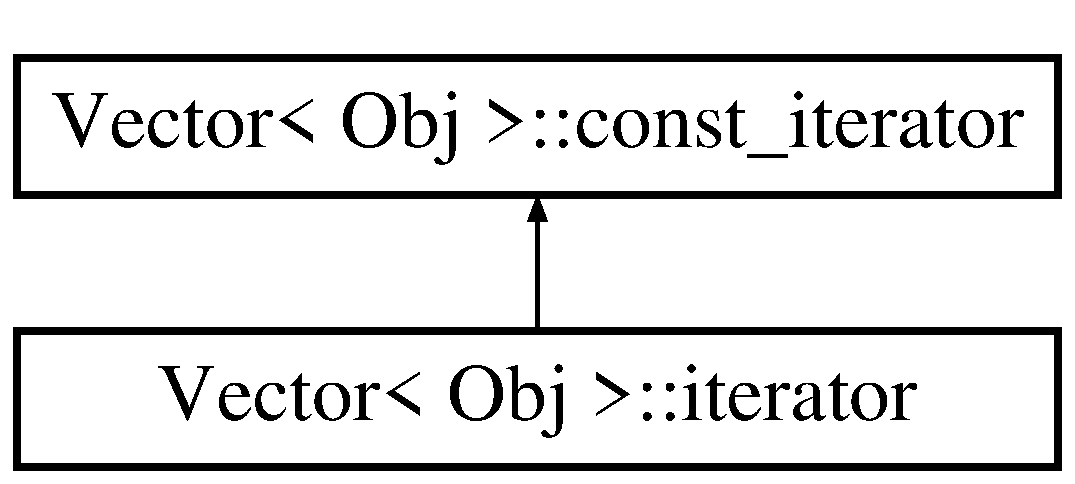
\includegraphics[height=2.000000cm]{class_vector_1_1iterator}
\end{center}
\end{figure}
\subsection*{Membros públicos}
\begin{DoxyCompactItemize}
\item 
\hyperlink{class_vector_1_1iterator_aa69868c2cdf276d8775e30fb905db3c1}{iterator} ()\hypertarget{class_vector_1_1iterator_aa69868c2cdf276d8775e30fb905db3c1}{}\label{class_vector_1_1iterator_aa69868c2cdf276d8775e30fb905db3c1}

\begin{DoxyCompactList}\small\item\em Construtor padrao. \end{DoxyCompactList}\item 
const Obj \& \hyperlink{class_vector_1_1iterator_a734abe09985e0d060a092fdd4e8fe56f}{operator$\ast$} () const \hypertarget{class_vector_1_1iterator_a734abe09985e0d060a092fdd4e8fe56f}{}\label{class_vector_1_1iterator_a734abe09985e0d060a092fdd4e8fe56f}

\begin{DoxyCompactList}\small\item\em Sobrecarga para o operador $\ast$. \end{DoxyCompactList}\item 
Obj \& \hyperlink{class_vector_1_1iterator_a489fefc64b8e2ce69631efc39713d75c}{operator$\ast$} ()\hypertarget{class_vector_1_1iterator_a489fefc64b8e2ce69631efc39713d75c}{}\label{class_vector_1_1iterator_a489fefc64b8e2ce69631efc39713d75c}

\begin{DoxyCompactList}\small\item\em Sobrecarga para o operador $\ast$. \end{DoxyCompactList}\item 
\hyperlink{class_vector_1_1iterator}{iterator} \& \hyperlink{class_vector_1_1iterator_a25f7b0fd1546c398727d588234f2abd6}{operator-\/-\/} ()\hypertarget{class_vector_1_1iterator_a25f7b0fd1546c398727d588234f2abd6}{}\label{class_vector_1_1iterator_a25f7b0fd1546c398727d588234f2abd6}

\begin{DoxyCompactList}\small\item\em Sobrecarga para o operador ++ (Infixo) \end{DoxyCompactList}\item 
\hyperlink{class_vector_1_1iterator}{iterator} \hyperlink{class_vector_1_1iterator_a1e2173dcc74c5d97ef0033b8400e2cff}{operator-\/-\/} (int)\hypertarget{class_vector_1_1iterator_a1e2173dcc74c5d97ef0033b8400e2cff}{}\label{class_vector_1_1iterator_a1e2173dcc74c5d97ef0033b8400e2cff}

\begin{DoxyCompactList}\small\item\em Sobrecarga para o operador ++ (Posfixo) \end{DoxyCompactList}\item 
\hyperlink{class_vector_1_1iterator}{iterator} \& \hyperlink{class_vector_1_1iterator_ab48c26866ff8e1792ed576cee7a41aca}{operator++} ()\hypertarget{class_vector_1_1iterator_ab48c26866ff8e1792ed576cee7a41aca}{}\label{class_vector_1_1iterator_ab48c26866ff8e1792ed576cee7a41aca}

\begin{DoxyCompactList}\small\item\em Sobrecarga para o operador ++ (Infixo) \end{DoxyCompactList}\item 
\hyperlink{class_vector_1_1iterator}{iterator} \hyperlink{class_vector_1_1iterator_a1c3d9ac3129b200ec59fe68de7dddaee}{operator++} (int)\hypertarget{class_vector_1_1iterator_a1c3d9ac3129b200ec59fe68de7dddaee}{}\label{class_vector_1_1iterator_a1c3d9ac3129b200ec59fe68de7dddaee}

\begin{DoxyCompactList}\small\item\em Sobrecarga para o operador ++ (Posfixo) \end{DoxyCompactList}\end{DoxyCompactItemize}
\subsection*{Membros protegidos}
\begin{DoxyCompactItemize}
\item 
{\bfseries iterator} (Obj $\ast$x)\hypertarget{class_vector_1_1iterator_a1d85d1cd4c77489a8db6fb5dd12b47f9}{}\label{class_vector_1_1iterator_a1d85d1cd4c77489a8db6fb5dd12b47f9}

\end{DoxyCompactItemize}
\subsection*{Amigos}
\begin{DoxyCompactItemize}
\item 
class {\bfseries Vector$<$ Obj $>$}\hypertarget{class_vector_1_1iterator_a93580d986919dca737b45fdf1c366bfa}{}\label{class_vector_1_1iterator_a93580d986919dca737b45fdf1c366bfa}

\end{DoxyCompactItemize}
\subsection*{Outros membros herdados}


A documentação para esta classe foi gerada a partir do seguinte ficheiro\+:\begin{DoxyCompactItemize}
\item 
V\+E\+C\+T\+O\+R/include/\hyperlink{vector_8h}{vector.\+h}\end{DoxyCompactItemize}

\hypertarget{class_list_1_1iterator}{}\section{Referência à classe List$<$ T $>$\+:\+:iterator}
\label{class_list_1_1iterator}\index{List$<$ T $>$\+::iterator@{List$<$ T $>$\+::iterator}}


Classe iterator.  




{\ttfamily \#include $<$list.\+h$>$}

Diagrama de heranças da classe List$<$ T $>$\+:\+:iterator\begin{figure}[H]
\begin{center}
\leavevmode
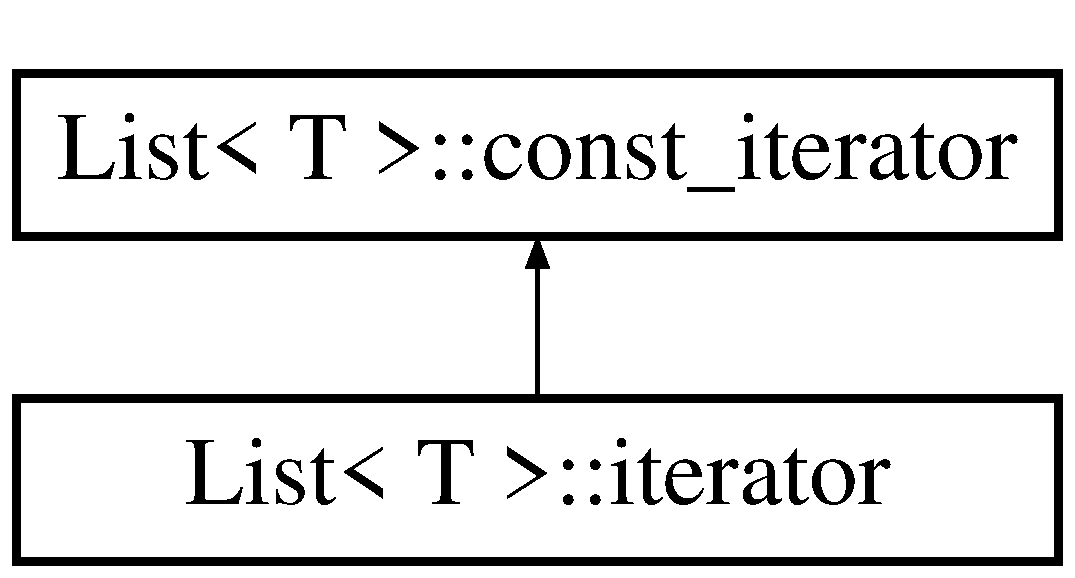
\includegraphics[height=2.000000cm]{class_list_1_1iterator}
\end{center}
\end{figure}
\subsection*{Membros públicos}
\begin{DoxyCompactItemize}
\item 
\hyperlink{class_list_1_1iterator_a90c7cf3543e4b139a6262d54a1f0fc63}{iterator} ()\hypertarget{class_list_1_1iterator_a90c7cf3543e4b139a6262d54a1f0fc63}{}\label{class_list_1_1iterator_a90c7cf3543e4b139a6262d54a1f0fc63}

\begin{DoxyCompactList}\small\item\em Construtor padrao. \end{DoxyCompactList}\item 
const T \& \hyperlink{class_list_1_1iterator_ad6d5f1650454631411d07996e892b017}{operator$\ast$} () const \hypertarget{class_list_1_1iterator_ad6d5f1650454631411d07996e892b017}{}\label{class_list_1_1iterator_ad6d5f1650454631411d07996e892b017}

\begin{DoxyCompactList}\small\item\em Sobrecarga para o operador $\ast$. \end{DoxyCompactList}\item 
T \& \hyperlink{class_list_1_1iterator_a24294112d6f9d39fa0353b6d81100d9c}{operator$\ast$} ()\hypertarget{class_list_1_1iterator_a24294112d6f9d39fa0353b6d81100d9c}{}\label{class_list_1_1iterator_a24294112d6f9d39fa0353b6d81100d9c}

\begin{DoxyCompactList}\small\item\em Sobrecarga para o operador $\ast$. \end{DoxyCompactList}\item 
\hyperlink{class_list_1_1iterator}{iterator} \& \hyperlink{class_list_1_1iterator_abc8967388edaaed0fa5414d79831d9c2}{operator++} ()\hypertarget{class_list_1_1iterator_abc8967388edaaed0fa5414d79831d9c2}{}\label{class_list_1_1iterator_abc8967388edaaed0fa5414d79831d9c2}

\begin{DoxyCompactList}\small\item\em Sobrecarga para o operador ++ (Infixo) \end{DoxyCompactList}\item 
\hyperlink{class_list_1_1iterator}{iterator} \hyperlink{class_list_1_1iterator_a03d5920ec99ec81284b4a622b4781e14}{operator++} (int)\hypertarget{class_list_1_1iterator_a03d5920ec99ec81284b4a622b4781e14}{}\label{class_list_1_1iterator_a03d5920ec99ec81284b4a622b4781e14}

\begin{DoxyCompactList}\small\item\em Sobrecarga para o operador ++ (Posfixo) \end{DoxyCompactList}\end{DoxyCompactItemize}
\subsection*{Membros protegidos}
\begin{DoxyCompactItemize}
\item 
{\bfseries iterator} (Node $\ast$p)\hypertarget{class_list_1_1iterator_a8500b544cba7bda0c19036391ea0fa7b}{}\label{class_list_1_1iterator_a8500b544cba7bda0c19036391ea0fa7b}

\end{DoxyCompactItemize}
\subsection*{Amigos}
\begin{DoxyCompactItemize}
\item 
class {\bfseries List$<$ T $>$}\hypertarget{class_list_1_1iterator_adfa51a0eca1eba953f68ca3f65cdaa05}{}\label{class_list_1_1iterator_adfa51a0eca1eba953f68ca3f65cdaa05}

\end{DoxyCompactItemize}
\subsection*{Outros membros herdados}


\subsection{Descrição detalhada}
\subsubsection*{template$<$typename T$>$\\*
class List$<$ T $>$\+::iterator}

Classe iterator. 

A documentação para esta classe foi gerada a partir do seguinte ficheiro\+:\begin{DoxyCompactItemize}
\item 
List/include/\hyperlink{list_8h}{list.\+h}\end{DoxyCompactItemize}

\hypertarget{class_forward__list_1_1iterator}{}\section{Referência à classe Forward\+\_\+list$<$ T $>$\+:\+:iterator}
\label{class_forward__list_1_1iterator}\index{Forward\+\_\+list$<$ T $>$\+::iterator@{Forward\+\_\+list$<$ T $>$\+::iterator}}


Classe iterator.  




{\ttfamily \#include $<$forward\+\_\+list.\+h$>$}

Diagrama de heranças da classe Forward\+\_\+list$<$ T $>$\+:\+:iterator\begin{figure}[H]
\begin{center}
\leavevmode
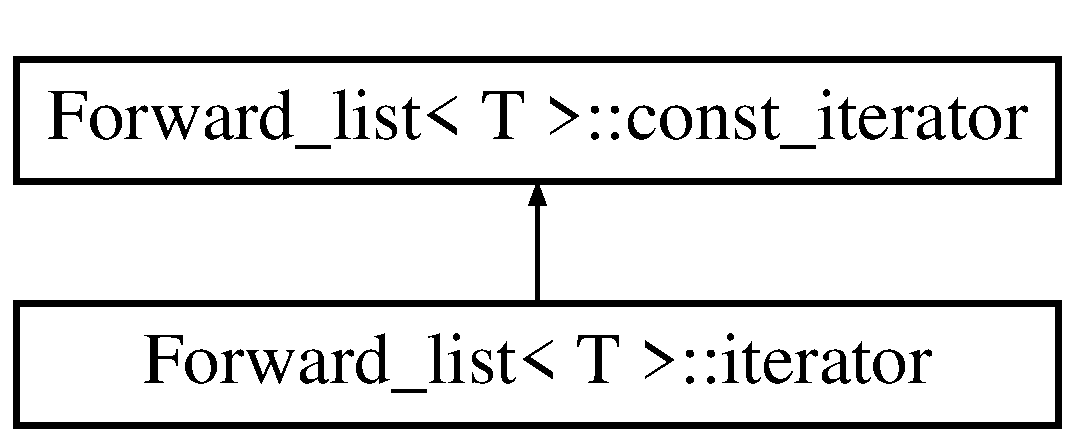
\includegraphics[height=2.000000cm]{class_forward__list_1_1iterator}
\end{center}
\end{figure}
\subsection*{Membros públicos}
\begin{DoxyCompactItemize}
\item 
\hyperlink{class_forward__list_1_1iterator_a969fbd51b73fadce7cb1d70374853d00}{iterator} ()\hypertarget{class_forward__list_1_1iterator_a969fbd51b73fadce7cb1d70374853d00}{}\label{class_forward__list_1_1iterator_a969fbd51b73fadce7cb1d70374853d00}

\begin{DoxyCompactList}\small\item\em Construtor padrao. \end{DoxyCompactList}\item 
const T \& \hyperlink{class_forward__list_1_1iterator_a29fa5d1fb4101a2eff9e69af91375cea}{operator$\ast$} () const \hypertarget{class_forward__list_1_1iterator_a29fa5d1fb4101a2eff9e69af91375cea}{}\label{class_forward__list_1_1iterator_a29fa5d1fb4101a2eff9e69af91375cea}

\begin{DoxyCompactList}\small\item\em Sobrecarga para o operador $\ast$. \end{DoxyCompactList}\item 
T \& \hyperlink{class_forward__list_1_1iterator_a7adb38a0c3fa47cd3f482093137b5286}{operator$\ast$} ()\hypertarget{class_forward__list_1_1iterator_a7adb38a0c3fa47cd3f482093137b5286}{}\label{class_forward__list_1_1iterator_a7adb38a0c3fa47cd3f482093137b5286}

\begin{DoxyCompactList}\small\item\em Sobrecarga para o operador $\ast$. \end{DoxyCompactList}\item 
\hyperlink{class_forward__list_1_1iterator}{iterator} \& \hyperlink{class_forward__list_1_1iterator_adc23300020d416752ff5c7bce13523ad}{operator++} ()\hypertarget{class_forward__list_1_1iterator_adc23300020d416752ff5c7bce13523ad}{}\label{class_forward__list_1_1iterator_adc23300020d416752ff5c7bce13523ad}

\begin{DoxyCompactList}\small\item\em Sobrecarga para o operador ++ (Infixo) \end{DoxyCompactList}\item 
\hyperlink{class_forward__list_1_1iterator}{iterator} \hyperlink{class_forward__list_1_1iterator_a6a0ccccd9b78ebdd72715e20b2fd62f4}{operator++} (int)\hypertarget{class_forward__list_1_1iterator_a6a0ccccd9b78ebdd72715e20b2fd62f4}{}\label{class_forward__list_1_1iterator_a6a0ccccd9b78ebdd72715e20b2fd62f4}

\begin{DoxyCompactList}\small\item\em Sobrecarga para o operador ++ (Posfixo) \end{DoxyCompactList}\end{DoxyCompactItemize}
\subsection*{Membros protegidos}
\begin{DoxyCompactItemize}
\item 
{\bfseries iterator} (Node $\ast$p)\hypertarget{class_forward__list_1_1iterator_a467fad82452066feaa38e615756b1c6e}{}\label{class_forward__list_1_1iterator_a467fad82452066feaa38e615756b1c6e}

\end{DoxyCompactItemize}
\subsection*{Amigos}
\begin{DoxyCompactItemize}
\item 
class {\bfseries Forward\+\_\+list$<$ T $>$}\hypertarget{class_forward__list_1_1iterator_a3248a6782762842dd0d50fa2ff16e968}{}\label{class_forward__list_1_1iterator_a3248a6782762842dd0d50fa2ff16e968}

\end{DoxyCompactItemize}
\subsection*{Outros membros herdados}


\subsection{Descrição detalhada}
\subsubsection*{template$<$typename T$>$\\*
class Forward\+\_\+list$<$ T $>$\+::iterator}

Classe iterator. 

A documentação para esta classe foi gerada a partir do seguinte ficheiro\+:\begin{DoxyCompactItemize}
\item 
Forward\+\_\+\+List/include/\hyperlink{forward__list_8h}{forward\+\_\+list.\+h}\end{DoxyCompactItemize}

\hypertarget{class_list}{}\section{Referência à classe Template List$<$ T $>$}
\label{class_list}\index{List$<$ T $>$@{List$<$ T $>$}}


Classe \hyperlink{class_list}{List}.  




{\ttfamily \#include $<$list.\+h$>$}

\subsection*{Componentes}
\begin{DoxyCompactItemize}
\item 
class \hyperlink{class_list_1_1const__iterator}{const\+\_\+iterator}
\item 
class \hyperlink{class_list_1_1iterator}{iterator}
\begin{DoxyCompactList}\small\item\em Classe iterator. \end{DoxyCompactList}\end{DoxyCompactItemize}
\subsection*{Membros públicos}
\begin{DoxyCompactItemize}
\item 
\hyperlink{class_list_a5c5e27671b21b3815d4e25b953c69454}{List} ()\hypertarget{class_list_a5c5e27671b21b3815d4e25b953c69454}{}\label{class_list_a5c5e27671b21b3815d4e25b953c69454}

\begin{DoxyCompactList}\small\item\em Construtor padrão da classe \hyperlink{class_list}{List} Seta os valores alocando novos nós. \end{DoxyCompactList}\item 
\hyperlink{class_list_a2b58189090f6e5ce52939c9195e59e85}{$\sim$\+List} ()\hypertarget{class_list_a2b58189090f6e5ce52939c9195e59e85}{}\label{class_list_a2b58189090f6e5ce52939c9195e59e85}

\begin{DoxyCompactList}\small\item\em Destrutor da classe \hyperlink{class_list}{List} Destroi o m\+\_\+head e o m\+\_\+tail. \end{DoxyCompactList}\item 
\hyperlink{class_list_a1d0f3740befe48d6e9db8d6b1320491a}{List} (const \hyperlink{class_list}{List} \&\+\_\+list)\hypertarget{class_list_a1d0f3740befe48d6e9db8d6b1320491a}{}\label{class_list_a1d0f3740befe48d6e9db8d6b1320491a}

\begin{DoxyCompactList}\small\item\em Construtor cópia da classe \hyperlink{class_list}{List} Faz uma cópia de todos os valores do objeto no qual se quer copiar. \end{DoxyCompactList}\item 
\hyperlink{class_list_a196fe489dad007c9734efdf94060f21c}{List} (\hyperlink{class_list}{List} \&\&\+\_\+list)\hypertarget{class_list_a196fe489dad007c9734efdf94060f21c}{}\label{class_list_a196fe489dad007c9734efdf94060f21c}

\begin{DoxyCompactList}\small\item\em Construtor move da classe \hyperlink{class_list}{List} Move todos os elementos de um objeto de uma classe para outro objeto. \end{DoxyCompactList}\item 
\hyperlink{class_list}{List} \& \hyperlink{class_list_a3a2c792d937e5df5ff9977853021feee}{operator=} (const \hyperlink{class_list}{List} \&\+\_\+list)
\begin{DoxyCompactList}\small\item\em Sobrecarga do operador cópia   $\ast$ @ Param list O elemento a ser copiado   $\ast$. \end{DoxyCompactList}\item 
\hyperlink{class_list}{List} \& \hyperlink{class_list_ad9b33c07a074c6cf4551f097d11f2739}{operator=} (\hyperlink{class_list}{List} \&\&\+\_\+list)
\begin{DoxyCompactList}\small\item\em Sobrecarga do operador move   $\ast$ @ Param list O elemento a ser movido   $\ast$. \end{DoxyCompactList}\item 
\hyperlink{class_list_1_1iterator}{iterator} \hyperlink{class_list_af5325bc089d1216204eba3d7febe68fd}{before\+\_\+begin} ()
\begin{DoxyCompactList}\small\item\em Pega um iterador apontando para o inicio da lista. \end{DoxyCompactList}\item 
\hyperlink{class_list_1_1iterator}{iterator} \hyperlink{class_list_a0826516313ad1e1bd48bfbb96bee618b}{begin} ()
\begin{DoxyCompactList}\small\item\em Pega um iterador apontando para o primeiro elemento da lista. \end{DoxyCompactList}\item 
\hyperlink{class_list_1_1iterator}{iterator} \hyperlink{class_list_ab18d47922493e508f89a0cf8c82fc4a0}{end} ()
\begin{DoxyCompactList}\small\item\em Pega um iterador apontando para o ultimo elemento da lista. \end{DoxyCompactList}\item 
\hyperlink{class_list_1_1const__iterator}{const\+\_\+iterator} \hyperlink{class_list_a4d03e75dc105d2c9ed6a1aa08c6a0eac}{cbefore\+\_\+begin} () const 
\begin{DoxyCompactList}\small\item\em Pega um iterador apontando para o inicio da lista. \end{DoxyCompactList}\item 
\hyperlink{class_list_1_1const__iterator}{const\+\_\+iterator} \hyperlink{class_list_a8affd35c61fccd7b4c7968d6c481fd27}{cbegin} () const 
\begin{DoxyCompactList}\small\item\em Pega um iterador const apontando para o primeiro elemento da lista. \end{DoxyCompactList}\item 
\hyperlink{class_list_1_1const__iterator}{const\+\_\+iterator} \hyperlink{class_list_af21c0053d502872bb1d14ab896e37f2e}{cend} () const 
\begin{DoxyCompactList}\small\item\em Pega um iterador const apontando para o ultimo elemento da lista. \end{DoxyCompactList}\item 
int \hyperlink{class_list_a802e2aa9aaef248591140fa032d20d61}{size} () const 
\begin{DoxyCompactList}\small\item\em Colhe o tamanho da lista. \end{DoxyCompactList}\item 
bool \hyperlink{class_list_ad96bf379b8e75539b20ad30d10f10269}{empty} () const 
\begin{DoxyCompactList}\small\item\em Verifica se a lista está vazia. \end{DoxyCompactList}\item 
void \hyperlink{class_list_ae296516a252e11963dbf963727ce429a}{clear} ()
\begin{DoxyCompactList}\small\item\em Deleta todos os elementos da lista. \end{DoxyCompactList}\item 
T \& \hyperlink{class_list_ad07fb4dd1af3e2b5335476d931417631}{front} ()
\begin{DoxyCompactList}\small\item\em Pega o elemento da frente da lista. \end{DoxyCompactList}\item 
const T \& \hyperlink{class_list_aa485ade02602d7594a76e78d2b1815bb}{front} () const 
\begin{DoxyCompactList}\small\item\em Pega o elemento da frente da lista. \end{DoxyCompactList}\item 
T \& \hyperlink{class_list_adcf79239b840f8600ea74e526120e69b}{back} ()
\begin{DoxyCompactList}\small\item\em Pega o elemento do final da lista. \end{DoxyCompactList}\item 
const T \& \hyperlink{class_list_a20e620772670fea9011193aa6e9caea5}{back} () const 
\begin{DoxyCompactList}\small\item\em Pega o elemento do final da lista. \end{DoxyCompactList}\item 
void \hyperlink{class_list_a2919a4bfce2d3ef66d13f64d5f722f4f}{push\+\_\+front} (const T \&x)
\begin{DoxyCompactList}\small\item\em Insere Elementos na frente da lista. \end{DoxyCompactList}\item 
void \hyperlink{class_list_ada56bf4c89094e9bbda854fc88cbacea}{push\+\_\+back} (const T \&x)
\begin{DoxyCompactList}\small\item\em Insere Elementos no final da lista. \end{DoxyCompactList}\item 
void \hyperlink{class_list_a024af4543f71544345351a45850c42d8}{pop\+\_\+front} ()
\begin{DoxyCompactList}\small\item\em Deleta Elementos na frente da lista. \end{DoxyCompactList}\item 
void \hyperlink{class_list_a42e1aee3e26b76b3f4d9386efa7fe8b7}{pop\+\_\+back} ()
\begin{DoxyCompactList}\small\item\em Deleta Elementos no final da lista. \end{DoxyCompactList}\item 
void \hyperlink{class_list_ab916628c8dd07761839b565ac533c6c7}{assign} (const T \&value)
\begin{DoxyCompactList}\small\item\em Insere o elemento em todas as posicoes da lista. \end{DoxyCompactList}\item 
void {\bfseries assign} (std\+::initializer\+\_\+list$<$ T $>$ ilist)\hypertarget{class_list_aa402aceaa13297356e19b1040f7852de}{}\label{class_list_aa402aceaa13297356e19b1040f7852de}

\item 
\hyperlink{class_list_1_1iterator}{iterator} \hyperlink{class_list_af5af80234fbd0b47a7fb85b2119e54ba}{insert\+\_\+after} (\hyperlink{class_list_1_1const__iterator}{const\+\_\+iterator} itr, const T \&x)
\begin{DoxyCompactList}\small\item\em Insere um elemento em uma posicao passada por parametro. \end{DoxyCompactList}\item 
\hyperlink{class_list_1_1iterator}{iterator} \hyperlink{class_list_a8d5b3bfe6314a321425b74632fc63ef8}{insert\+\_\+after} (\hyperlink{class_list_1_1const__iterator}{const\+\_\+iterator} pos, std\+::initializer\+\_\+list$<$ T $>$ ilist)
\begin{DoxyCompactList}\small\item\em Insere uma lista na lista iterador passada por parametro. \end{DoxyCompactList}\item 
\hyperlink{class_list_1_1iterator}{iterator} \hyperlink{class_list_a901409fcfd7cb1e04aeaf213fe613a4d}{erase\+\_\+after} (\hyperlink{class_list_1_1const__iterator}{const\+\_\+iterator} itr)
\begin{DoxyCompactList}\small\item\em Apaga um elemento em uma posicao passada por parametro. \end{DoxyCompactList}\item 
\hyperlink{class_list_1_1iterator}{iterator} \hyperlink{class_list_a3e1572fd28739327efe18b41f23c2079}{erase\+\_\+after} (\hyperlink{class_list_1_1const__iterator}{const\+\_\+iterator} first, \hyperlink{class_list_1_1const__iterator}{const\+\_\+iterator} last)
\begin{DoxyCompactList}\small\item\em Apaga os elementos em um intervalo passado por parametro. \end{DoxyCompactList}\item 
\hyperlink{class_list_1_1const__iterator}{const\+\_\+iterator} \hyperlink{class_list_a23e3b812e8ce38d728a036fb7bffc368}{find} (const T \&x) const 
\begin{DoxyCompactList}\small\item\em Procura um elemento na lista. \end{DoxyCompactList}\end{DoxyCompactItemize}


\subsection{Descrição detalhada}
\subsubsection*{template$<$typename T$>$\\*
class List$<$ T $>$}

Classe \hyperlink{class_list}{List}. 

Assinaturas das funções e definição da classe \hyperlink{class_list}{List} 

\subsection{Documentação dos métodos}
\index{List@{List}!assign@{assign}}
\index{assign@{assign}!List@{List}}
\subsubsection[{\texorpdfstring{assign(const T \&value)}{assign(const T &value)}}]{\setlength{\rightskip}{0pt plus 5cm}template$<$typename T $>$ void {\bf List}$<$ T $>$\+::assign (
\begin{DoxyParamCaption}
\item[{const T \&}]{value}
\end{DoxyParamCaption}
)}\hypertarget{class_list_ab916628c8dd07761839b565ac533c6c7}{}\label{class_list_ab916628c8dd07761839b565ac533c6c7}


Insere o elemento em todas as posicoes da lista. 


\begin{DoxyParams}{Parâmetros}
{\em value} & Elemento a ser inserido \\
\hline
\end{DoxyParams}
\begin{DoxyReturn}{Retorna}
void 
\end{DoxyReturn}
\index{List@{List}!back@{back}}
\index{back@{back}!List@{List}}
\subsubsection[{\texorpdfstring{back()}{back()}}]{\setlength{\rightskip}{0pt plus 5cm}template$<$typename T $>$ T \& {\bf List}$<$ T $>$\+::back (
\begin{DoxyParamCaption}
{}
\end{DoxyParamCaption}
)}\hypertarget{class_list_adcf79239b840f8600ea74e526120e69b}{}\label{class_list_adcf79239b840f8600ea74e526120e69b}


Pega o elemento do final da lista. 

\begin{DoxyReturn}{Retorna}
A referência para o ultimo elemento 
\end{DoxyReturn}
\index{List@{List}!back@{back}}
\index{back@{back}!List@{List}}
\subsubsection[{\texorpdfstring{back() const }{back() const }}]{\setlength{\rightskip}{0pt plus 5cm}template$<$typename T $>$ const T \& {\bf List}$<$ T $>$\+::back (
\begin{DoxyParamCaption}
{}
\end{DoxyParamCaption}
) const}\hypertarget{class_list_a20e620772670fea9011193aa6e9caea5}{}\label{class_list_a20e620772670fea9011193aa6e9caea5}


Pega o elemento do final da lista. 

\begin{DoxyReturn}{Retorna}
A referência const para o ultimo elemento 
\end{DoxyReturn}
\index{List@{List}!before\+\_\+begin@{before\+\_\+begin}}
\index{before\+\_\+begin@{before\+\_\+begin}!List@{List}}
\subsubsection[{\texorpdfstring{before\+\_\+begin()}{before_begin()}}]{\setlength{\rightskip}{0pt plus 5cm}template$<$typename T $>$ {\bf List}$<$ T $>$\+::{\bf iterator} {\bf List}$<$ T $>$\+::before\+\_\+begin (
\begin{DoxyParamCaption}
{}
\end{DoxyParamCaption}
)}\hypertarget{class_list_af5325bc089d1216204eba3d7febe68fd}{}\label{class_list_af5325bc089d1216204eba3d7febe68fd}


Pega um iterador apontando para o inicio da lista. 

  $\ast$ \begin{DoxyReturn}{Retorna}
Um iterador para o inicio da lista 
\end{DoxyReturn}
\index{List@{List}!begin@{begin}}
\index{begin@{begin}!List@{List}}
\subsubsection[{\texorpdfstring{begin()}{begin()}}]{\setlength{\rightskip}{0pt plus 5cm}template$<$typename T $>$ {\bf List}$<$ T $>$\+::{\bf iterator} {\bf List}$<$ T $>$\+::begin (
\begin{DoxyParamCaption}
{}
\end{DoxyParamCaption}
)}\hypertarget{class_list_a0826516313ad1e1bd48bfbb96bee618b}{}\label{class_list_a0826516313ad1e1bd48bfbb96bee618b}


Pega um iterador apontando para o primeiro elemento da lista. 

  $\ast$ \begin{DoxyReturn}{Retorna}
Um iterador apontando para o primeiro elemento da lista 
\end{DoxyReturn}
\index{List@{List}!cbefore\+\_\+begin@{cbefore\+\_\+begin}}
\index{cbefore\+\_\+begin@{cbefore\+\_\+begin}!List@{List}}
\subsubsection[{\texorpdfstring{cbefore\+\_\+begin() const }{cbefore_begin() const }}]{\setlength{\rightskip}{0pt plus 5cm}template$<$typename T $>$ {\bf List}$<$ T $>$\+::{\bf const\+\_\+iterator} {\bf List}$<$ T $>$\+::cbefore\+\_\+begin (
\begin{DoxyParamCaption}
{}
\end{DoxyParamCaption}
) const}\hypertarget{class_list_a4d03e75dc105d2c9ed6a1aa08c6a0eac}{}\label{class_list_a4d03e75dc105d2c9ed6a1aa08c6a0eac}


Pega um iterador apontando para o inicio da lista. 

  $\ast$ \begin{DoxyReturn}{Retorna}
Um iterador para o inicio da lista 
\end{DoxyReturn}
\index{List@{List}!cbegin@{cbegin}}
\index{cbegin@{cbegin}!List@{List}}
\subsubsection[{\texorpdfstring{cbegin() const }{cbegin() const }}]{\setlength{\rightskip}{0pt plus 5cm}template$<$typename T $>$ {\bf List}$<$ T $>$\+::{\bf const\+\_\+iterator} {\bf List}$<$ T $>$\+::cbegin (
\begin{DoxyParamCaption}
{}
\end{DoxyParamCaption}
) const}\hypertarget{class_list_a8affd35c61fccd7b4c7968d6c481fd27}{}\label{class_list_a8affd35c61fccd7b4c7968d6c481fd27}


Pega um iterador const apontando para o primeiro elemento da lista. 

  $\ast$ \begin{DoxyReturn}{Retorna}
Um iterador apontando para o primeiro elemento da lista 
\end{DoxyReturn}
\index{List@{List}!cend@{cend}}
\index{cend@{cend}!List@{List}}
\subsubsection[{\texorpdfstring{cend() const }{cend() const }}]{\setlength{\rightskip}{0pt plus 5cm}template$<$typename T $>$ {\bf List}$<$ T $>$\+::{\bf const\+\_\+iterator} {\bf List}$<$ T $>$\+::cend (
\begin{DoxyParamCaption}
{}
\end{DoxyParamCaption}
) const}\hypertarget{class_list_af21c0053d502872bb1d14ab896e37f2e}{}\label{class_list_af21c0053d502872bb1d14ab896e37f2e}


Pega um iterador const apontando para o ultimo elemento da lista. 

  $\ast$ \begin{DoxyReturn}{Retorna}
Um iterador apontando para o ultimo elemento da lista 
\end{DoxyReturn}
\index{List@{List}!clear@{clear}}
\index{clear@{clear}!List@{List}}
\subsubsection[{\texorpdfstring{clear()}{clear()}}]{\setlength{\rightskip}{0pt plus 5cm}template$<$typename T $>$ void {\bf List}$<$ T $>$\+::clear (
\begin{DoxyParamCaption}
{}
\end{DoxyParamCaption}
)}\hypertarget{class_list_ae296516a252e11963dbf963727ce429a}{}\label{class_list_ae296516a252e11963dbf963727ce429a}


Deleta todos os elementos da lista. 

\begin{DoxyReturn}{Retorna}
void 
\end{DoxyReturn}
\index{List@{List}!empty@{empty}}
\index{empty@{empty}!List@{List}}
\subsubsection[{\texorpdfstring{empty() const }{empty() const }}]{\setlength{\rightskip}{0pt plus 5cm}template$<$typename T $>$ bool {\bf List}$<$ T $>$\+::empty (
\begin{DoxyParamCaption}
{}
\end{DoxyParamCaption}
) const}\hypertarget{class_list_ad96bf379b8e75539b20ad30d10f10269}{}\label{class_list_ad96bf379b8e75539b20ad30d10f10269}


Verifica se a lista está vazia. 

\begin{DoxyReturn}{Retorna}
True se estiver vazia, ou False se não estiver vazia 
\end{DoxyReturn}
\index{List@{List}!end@{end}}
\index{end@{end}!List@{List}}
\subsubsection[{\texorpdfstring{end()}{end()}}]{\setlength{\rightskip}{0pt plus 5cm}template$<$typename T $>$ {\bf List}$<$ T $>$\+::{\bf iterator} {\bf List}$<$ T $>$\+::end (
\begin{DoxyParamCaption}
{}
\end{DoxyParamCaption}
)}\hypertarget{class_list_ab18d47922493e508f89a0cf8c82fc4a0}{}\label{class_list_ab18d47922493e508f89a0cf8c82fc4a0}


Pega um iterador apontando para o ultimo elemento da lista. 

  $\ast$ \begin{DoxyReturn}{Retorna}
Um iterador apontando para o ultimo elemento da lista 
\end{DoxyReturn}
\index{List@{List}!erase\+\_\+after@{erase\+\_\+after}}
\index{erase\+\_\+after@{erase\+\_\+after}!List@{List}}
\subsubsection[{\texorpdfstring{erase\+\_\+after(const\+\_\+iterator itr)}{erase_after(const_iterator itr)}}]{\setlength{\rightskip}{0pt plus 5cm}template$<$typename T $>$ {\bf List}$<$ T $>$\+::{\bf iterator} {\bf List}$<$ T $>$\+::erase\+\_\+after (
\begin{DoxyParamCaption}
\item[{{\bf const\+\_\+iterator}}]{itr}
\end{DoxyParamCaption}
)}\hypertarget{class_list_a901409fcfd7cb1e04aeaf213fe613a4d}{}\label{class_list_a901409fcfd7cb1e04aeaf213fe613a4d}


Apaga um elemento em uma posicao passada por parametro. 


\begin{DoxyParams}{Parâmetros}
{\em itr} & O iterador para posicao a ser apagada \\
\hline
\end{DoxyParams}
\begin{DoxyReturn}{Retorna}
A posicao do elemento apagado 
\end{DoxyReturn}
\index{List@{List}!erase\+\_\+after@{erase\+\_\+after}}
\index{erase\+\_\+after@{erase\+\_\+after}!List@{List}}
\subsubsection[{\texorpdfstring{erase\+\_\+after(const\+\_\+iterator first, const\+\_\+iterator last)}{erase_after(const_iterator first, const_iterator last)}}]{\setlength{\rightskip}{0pt plus 5cm}template$<$typename T $>$ {\bf List}$<$ T $>$\+::{\bf iterator} {\bf List}$<$ T $>$\+::erase\+\_\+after (
\begin{DoxyParamCaption}
\item[{{\bf const\+\_\+iterator}}]{first, }
\item[{{\bf const\+\_\+iterator}}]{last}
\end{DoxyParamCaption}
)}\hypertarget{class_list_a3e1572fd28739327efe18b41f23c2079}{}\label{class_list_a3e1572fd28739327efe18b41f23c2079}


Apaga os elementos em um intervalo passado por parametro. 


\begin{DoxyParams}{Parâmetros}
{\em first} & O iterador para primeira posicao a ser apagada \\
\hline
{\em last} & O iterador para ultima posicao a ser apagada \\
\hline
\end{DoxyParams}
\begin{DoxyReturn}{Retorna}
A posicao do ultimo elemento apagado 
\end{DoxyReturn}
\index{List@{List}!find@{find}}
\index{find@{find}!List@{List}}
\subsubsection[{\texorpdfstring{find(const T \&x) const }{find(const T &x) const }}]{\setlength{\rightskip}{0pt plus 5cm}template$<$typename T $>$ {\bf List}$<$ T $>$\+::{\bf const\+\_\+iterator} {\bf List}$<$ T $>$\+::find (
\begin{DoxyParamCaption}
\item[{const T \&}]{x}
\end{DoxyParamCaption}
) const}\hypertarget{class_list_a23e3b812e8ce38d728a036fb7bffc368}{}\label{class_list_a23e3b812e8ce38d728a036fb7bffc368}


Procura um elemento na lista. 


\begin{DoxyParams}{Parâmetros}
{\em x} & O elemento a ser procurado \\
\hline
\end{DoxyParams}
\begin{DoxyReturn}{Retorna}
Um Iterador const para o elemento encontrado 
\end{DoxyReturn}
\index{List@{List}!front@{front}}
\index{front@{front}!List@{List}}
\subsubsection[{\texorpdfstring{front()}{front()}}]{\setlength{\rightskip}{0pt plus 5cm}template$<$typename T $>$ T \& {\bf List}$<$ T $>$\+::front (
\begin{DoxyParamCaption}
{}
\end{DoxyParamCaption}
)}\hypertarget{class_list_ad07fb4dd1af3e2b5335476d931417631}{}\label{class_list_ad07fb4dd1af3e2b5335476d931417631}


Pega o elemento da frente da lista. 

\begin{DoxyReturn}{Retorna}
A referência para o primeiro elemento 
\end{DoxyReturn}
\index{List@{List}!front@{front}}
\index{front@{front}!List@{List}}
\subsubsection[{\texorpdfstring{front() const }{front() const }}]{\setlength{\rightskip}{0pt plus 5cm}template$<$typename T $>$ const T \& {\bf List}$<$ T $>$\+::front (
\begin{DoxyParamCaption}
{}
\end{DoxyParamCaption}
) const}\hypertarget{class_list_aa485ade02602d7594a76e78d2b1815bb}{}\label{class_list_aa485ade02602d7594a76e78d2b1815bb}


Pega o elemento da frente da lista. 

\begin{DoxyReturn}{Retorna}
A referência const para o primeiro elemento 
\end{DoxyReturn}
\index{List@{List}!insert\+\_\+after@{insert\+\_\+after}}
\index{insert\+\_\+after@{insert\+\_\+after}!List@{List}}
\subsubsection[{\texorpdfstring{insert\+\_\+after(const\+\_\+iterator itr, const T \&x)}{insert_after(const_iterator itr, const T &x)}}]{\setlength{\rightskip}{0pt plus 5cm}template$<$typename T $>$ {\bf List}$<$ T $>$\+::{\bf iterator} {\bf List}$<$ T $>$\+::insert\+\_\+after (
\begin{DoxyParamCaption}
\item[{{\bf const\+\_\+iterator}}]{itr, }
\item[{const T \&}]{x}
\end{DoxyParamCaption}
)}\hypertarget{class_list_af5af80234fbd0b47a7fb85b2119e54ba}{}\label{class_list_af5af80234fbd0b47a7fb85b2119e54ba}


Insere um elemento em uma posicao passada por parametro. 


\begin{DoxyParams}{Parâmetros}
{\em itr} & O iterador para posicao a ser inserido o elemento \\
\hline
{\em x} & O elemento a ser inserido \\
\hline
\end{DoxyParams}
\begin{DoxyReturn}{Retorna}
O iterador para o elemento inserido 
\end{DoxyReturn}
\index{List@{List}!insert\+\_\+after@{insert\+\_\+after}}
\index{insert\+\_\+after@{insert\+\_\+after}!List@{List}}
\subsubsection[{\texorpdfstring{insert\+\_\+after(const\+\_\+iterator pos, std\+::initializer\+\_\+list$<$ T $>$ ilist)}{insert_after(const_iterator pos, std::initializer_list< T > ilist)}}]{\setlength{\rightskip}{0pt plus 5cm}template$<$typename T $>$ {\bf List}$<$ T $>$\+::{\bf iterator} {\bf List}$<$ T $>$\+::insert\+\_\+after (
\begin{DoxyParamCaption}
\item[{{\bf const\+\_\+iterator}}]{pos, }
\item[{std\+::initializer\+\_\+list$<$ T $>$}]{ilist}
\end{DoxyParamCaption}
)}\hypertarget{class_list_a8d5b3bfe6314a321425b74632fc63ef8}{}\label{class_list_a8d5b3bfe6314a321425b74632fc63ef8}


Insere uma lista na lista iterador passada por parametro. 


\begin{DoxyParams}{Parâmetros}
{\em pos} & O iterador para posicao a ser inserido o elemento \\
\hline
{\em ilist} & A lista a ser inserida \\
\hline
\end{DoxyParams}
\begin{DoxyReturn}{Retorna}
O iterador para o ultimo elemento adicionado 
\end{DoxyReturn}
\index{List@{List}!operator=@{operator=}}
\index{operator=@{operator=}!List@{List}}
\subsubsection[{\texorpdfstring{operator=(const List \&\+\_\+list)}{operator=(const List &_list)}}]{\setlength{\rightskip}{0pt plus 5cm}template$<$typename T $>$ {\bf List}\& {\bf List}$<$ T $>$\+::operator= (
\begin{DoxyParamCaption}
\item[{const {\bf List}$<$ T $>$ \&}]{\+\_\+list}
\end{DoxyParamCaption}
)\hspace{0.3cm}{\ttfamily [inline]}}\hypertarget{class_list_a3a2c792d937e5df5ff9977853021feee}{}\label{class_list_a3a2c792d937e5df5ff9977853021feee}


Sobrecarga do operador cópia   $\ast$ @ Param list O elemento a ser copiado   $\ast$. 

  $\ast$ \begin{DoxyReturn}{Retorna}
O this do elemento copiado   
\end{DoxyReturn}
\index{List@{List}!operator=@{operator=}}
\index{operator=@{operator=}!List@{List}}
\subsubsection[{\texorpdfstring{operator=(\+List \&\&\+\_\+list)}{operator=(List &&_list)}}]{\setlength{\rightskip}{0pt plus 5cm}template$<$typename T $>$ {\bf List}\& {\bf List}$<$ T $>$\+::operator= (
\begin{DoxyParamCaption}
\item[{{\bf List}$<$ T $>$ \&\&}]{\+\_\+list}
\end{DoxyParamCaption}
)\hspace{0.3cm}{\ttfamily [inline]}}\hypertarget{class_list_ad9b33c07a074c6cf4551f097d11f2739}{}\label{class_list_ad9b33c07a074c6cf4551f097d11f2739}


Sobrecarga do operador move   $\ast$ @ Param list O elemento a ser movido   $\ast$. 

  $\ast$ \begin{DoxyReturn}{Retorna}
O this do elemento movido   
\end{DoxyReturn}
\index{List@{List}!pop\+\_\+back@{pop\+\_\+back}}
\index{pop\+\_\+back@{pop\+\_\+back}!List@{List}}
\subsubsection[{\texorpdfstring{pop\+\_\+back()}{pop_back()}}]{\setlength{\rightskip}{0pt plus 5cm}template$<$typename T $>$ void {\bf List}$<$ T $>$\+::pop\+\_\+back (
\begin{DoxyParamCaption}
{}
\end{DoxyParamCaption}
)}\hypertarget{class_list_a42e1aee3e26b76b3f4d9386efa7fe8b7}{}\label{class_list_a42e1aee3e26b76b3f4d9386efa7fe8b7}


Deleta Elementos no final da lista. 

\begin{DoxyReturn}{Retorna}
void 
\end{DoxyReturn}
\index{List@{List}!pop\+\_\+front@{pop\+\_\+front}}
\index{pop\+\_\+front@{pop\+\_\+front}!List@{List}}
\subsubsection[{\texorpdfstring{pop\+\_\+front()}{pop_front()}}]{\setlength{\rightskip}{0pt plus 5cm}template$<$typename T $>$ void {\bf List}$<$ T $>$\+::pop\+\_\+front (
\begin{DoxyParamCaption}
{}
\end{DoxyParamCaption}
)}\hypertarget{class_list_a024af4543f71544345351a45850c42d8}{}\label{class_list_a024af4543f71544345351a45850c42d8}


Deleta Elementos na frente da lista. 

\begin{DoxyReturn}{Retorna}
void 
\end{DoxyReturn}
\index{List@{List}!push\+\_\+back@{push\+\_\+back}}
\index{push\+\_\+back@{push\+\_\+back}!List@{List}}
\subsubsection[{\texorpdfstring{push\+\_\+back(const T \&x)}{push_back(const T &x)}}]{\setlength{\rightskip}{0pt plus 5cm}template$<$typename T $>$ void {\bf List}$<$ T $>$\+::push\+\_\+back (
\begin{DoxyParamCaption}
\item[{const T \&}]{x}
\end{DoxyParamCaption}
)}\hypertarget{class_list_ada56bf4c89094e9bbda854fc88cbacea}{}\label{class_list_ada56bf4c89094e9bbda854fc88cbacea}


Insere Elementos no final da lista. 


\begin{DoxyParams}{Parâmetros}
{\em x} & O elemento a ser inserido \\
\hline
\end{DoxyParams}
\begin{DoxyReturn}{Retorna}
void 
\end{DoxyReturn}
\index{List@{List}!push\+\_\+front@{push\+\_\+front}}
\index{push\+\_\+front@{push\+\_\+front}!List@{List}}
\subsubsection[{\texorpdfstring{push\+\_\+front(const T \&x)}{push_front(const T &x)}}]{\setlength{\rightskip}{0pt plus 5cm}template$<$typename T $>$ void {\bf List}$<$ T $>$\+::push\+\_\+front (
\begin{DoxyParamCaption}
\item[{const T \&}]{x}
\end{DoxyParamCaption}
)}\hypertarget{class_list_a2919a4bfce2d3ef66d13f64d5f722f4f}{}\label{class_list_a2919a4bfce2d3ef66d13f64d5f722f4f}


Insere Elementos na frente da lista. 


\begin{DoxyParams}{Parâmetros}
{\em x} & O elemento a ser inserido \\
\hline
\end{DoxyParams}
\begin{DoxyReturn}{Retorna}
void 
\end{DoxyReturn}
\index{List@{List}!size@{size}}
\index{size@{size}!List@{List}}
\subsubsection[{\texorpdfstring{size() const }{size() const }}]{\setlength{\rightskip}{0pt plus 5cm}template$<$typename T $>$ int {\bf List}$<$ T $>$\+::size (
\begin{DoxyParamCaption}
{}
\end{DoxyParamCaption}
) const}\hypertarget{class_list_a802e2aa9aaef248591140fa032d20d61}{}\label{class_list_a802e2aa9aaef248591140fa032d20d61}


Colhe o tamanho da lista. 

\begin{DoxyReturn}{Retorna}
O tamanho da Forward list 
\end{DoxyReturn}


A documentação para esta classe foi gerada a partir dos seguintes ficheiros\+:\begin{DoxyCompactItemize}
\item 
List/include/\hyperlink{list_8h}{list.\+h}\item 
List/include/\hyperlink{list_8inl}{list.\+inl}\end{DoxyCompactItemize}

\hypertarget{class_vector}{}\section{Referência à classe Template Vector$<$ Obj $>$}
\label{class_vector}\index{Vector$<$ Obj $>$@{Vector$<$ Obj $>$}}


Classe \hyperlink{class_vector}{Vector}.  




{\ttfamily \#include $<$vector.\+h$>$}

\subsection*{Componentes}
\begin{DoxyCompactItemize}
\item 
class \hyperlink{class_vector_1_1const__iterator}{const\+\_\+iterator}
\item 
class \hyperlink{class_vector_1_1iterator}{iterator}
\end{DoxyCompactItemize}
\subsection*{Membros públicos}
\begin{DoxyCompactItemize}
\item 
\hyperlink{class_vector_a882e1f7a7fcb08d248bd2fa3f9869527}{Vector} (size\+\_\+t x=1)\hypertarget{class_vector_a882e1f7a7fcb08d248bd2fa3f9869527}{}\label{class_vector_a882e1f7a7fcb08d248bd2fa3f9869527}

\begin{DoxyCompactList}\small\item\em Construtor \hyperlink{class_vector}{Vector} @ Param x O tamanho do vetor. \end{DoxyCompactList}\item 
\hyperlink{class_vector_a42105d30af4b2da75975561e1aff74c4}{$\sim$\+Vector} ()\hypertarget{class_vector_a42105d30af4b2da75975561e1aff74c4}{}\label{class_vector_a42105d30af4b2da75975561e1aff74c4}

\begin{DoxyCompactList}\small\item\em Destrutor \hyperlink{class_vector}{Vector}. \end{DoxyCompactList}\item 
size\+\_\+t \hyperlink{class_vector_afe1de779df754eedd2a8a0be4d796643}{size} () const 
\begin{DoxyCompactList}\small\item\em Pega tamanho \hyperlink{class_vector}{Vector}   $\ast$. \end{DoxyCompactList}\item 
void \hyperlink{class_vector_ae7234417f87946c4bfcccf738af75837}{clear} ()
\begin{DoxyCompactList}\small\item\em Remove todos os elementos do vetor   \end{DoxyCompactList}\item 
bool \hyperlink{class_vector_a7d4b2337c2da133cc4868ce755730644}{empty} ()
\begin{DoxyCompactList}\small\item\em Verifica se o vetor está vazio   $\ast$. \end{DoxyCompactList}\item 
void \hyperlink{class_vector_a0edf2c3ff13e5c83ddea6ee5c8c8ec4f}{push\+\_\+back} (const Obj \&x)
\begin{DoxyCompactList}\small\item\em Adicionar um elemento no final do vector   $\ast$ @ Param x Elemento a ser colocado atrás    \end{DoxyCompactList}\item 
void \hyperlink{class_vector_a616d10a9af01df582450d1ba6fd2e1bc}{pop\+\_\+back} ()
\begin{DoxyCompactList}\small\item\em Remove o ultimo elemento do vetor    \end{DoxyCompactList}\item 
const Obj \& \hyperlink{class_vector_a239e09c772177108354d25fea6974bbd}{front} () const 
\begin{DoxyCompactList}\small\item\em Retorna o Obj no inicio do \hyperlink{class_vector}{Vector}   $\ast$. \end{DoxyCompactList}\item 
const Obj \& \hyperlink{class_vector_a67d8538b1d68f7a099622383565839d9}{back} () const 
\begin{DoxyCompactList}\small\item\em Retorna o Obj no fim do \hyperlink{class_vector}{Vector}   $\ast$. \end{DoxyCompactList}\item 
void \hyperlink{class_vector_a76ac292de41a52ebc948432c1220d13e}{assign} (const Obj \&x)
\begin{DoxyCompactList}\small\item\em Substitui o conteúdo do vetor   $\ast$ @ Param x Atribui novos conteúdos ao vector, substituindo seu conteúdo atual, e modificando seu tamanho em conformidade. \end{DoxyCompactList}\item 
size\+\_\+t \hyperlink{class_vector_acf2e59a5ce4f1059e08139989ece3e0b}{capacity} () const 
\begin{DoxyCompactList}\small\item\em Retorna a capacidade \hyperlink{class_vector}{Vector}   $\ast$. \end{DoxyCompactList}\item 
void \hyperlink{class_vector_a1a858089a6bc82faffabdeb03386a85f}{reserve} (size\+\_\+t new\+\_\+capacidade)
\begin{DoxyCompactList}\small\item\em Define a nova capacidade \hyperlink{class_vector}{Vector}   $\ast$ @ Param new\+\_\+capacidade O novo tamanho da capacidade    \end{DoxyCompactList}\item 
Obj \& \hyperlink{class_vector_a568255f8d17d285793167b1cee11f926}{at} (size\+\_\+t x)
\begin{DoxyCompactList}\small\item\em Retorna o elemento em alguma posição   $\ast$ @ Param x A posição a ser devolvido   $\ast$. \end{DoxyCompactList}\item 
Obj \& \hyperlink{class_vector_a51289cefc80dbd081f815f30a554b7db}{operator\mbox{[}$\,$\mbox{]}} (size\+\_\+t x)
\begin{DoxyCompactList}\small\item\em Sobrecarrega o operador \mbox{[}\mbox{]}   $\ast$ @ Param x posição a ser acessada   $\ast$. \end{DoxyCompactList}\item 
\hyperlink{class_vector_1_1const__iterator}{const\+\_\+iterator} \hyperlink{class_vector_a66c90ea54c76cf19aee525ed7f4c46dc}{cbegin} () const 
\begin{DoxyCompactList}\small\item\em Pega um iterador const apontando para o primeiro elemento da lista. \end{DoxyCompactList}\item 
\hyperlink{class_vector_1_1iterator}{iterator} \hyperlink{class_vector_a261d7f78f5ac7b890eff45ce86e8d58c}{begin} ()
\begin{DoxyCompactList}\small\item\em Pega um iterador apontando para o primeiro elemento da lista. \end{DoxyCompactList}\item 
\hyperlink{class_vector_1_1const__iterator}{const\+\_\+iterator} \hyperlink{class_vector_a300b3851da687ddfee9d3fcec7b1ebfc}{cend} () const 
\begin{DoxyCompactList}\small\item\em Pega um iterador const apontando para o ultimo elemento da lista. \end{DoxyCompactList}\item 
\hyperlink{class_vector_1_1iterator}{iterator} \hyperlink{class_vector_af0f2938e008aa9fe309d4b2af8dd4f11}{end} ()
\begin{DoxyCompactList}\small\item\em Pega um iterador apontando para o ultimo elemento da lista. \end{DoxyCompactList}\end{DoxyCompactItemize}


\subsection{Descrição detalhada}
\subsubsection*{template$<$typename Obj$>$\\*
class Vector$<$ Obj $>$}

Classe \hyperlink{class_vector}{Vector}. 

Assinaturas das funções e definição da classe \hyperlink{class_vector}{Vector} 

\subsection{Documentação dos métodos}
\index{Vector@{Vector}!assign@{assign}}
\index{assign@{assign}!Vector@{Vector}}
\subsubsection[{\texorpdfstring{assign(const Obj \&x)}{assign(const Obj &x)}}]{\setlength{\rightskip}{0pt plus 5cm}template$<$typename Obj $>$ void {\bf Vector}$<$ Obj $>$\+::assign (
\begin{DoxyParamCaption}
\item[{const Obj \&}]{x}
\end{DoxyParamCaption}
)}\hypertarget{class_vector_a76ac292de41a52ebc948432c1220d13e}{}\label{class_vector_a76ac292de41a52ebc948432c1220d13e}


Substitui o conteúdo do vetor   $\ast$ @ Param x Atribui novos conteúdos ao vector, substituindo seu conteúdo atual, e modificando seu tamanho em conformidade. 

  $\ast$ \index{Vector@{Vector}!at@{at}}
\index{at@{at}!Vector@{Vector}}
\subsubsection[{\texorpdfstring{at(size\+\_\+t x)}{at(size_t x)}}]{\setlength{\rightskip}{0pt plus 5cm}template$<$typename Obj $>$ Obj \& {\bf Vector}$<$ Obj $>$\+::at (
\begin{DoxyParamCaption}
\item[{size\+\_\+t}]{x}
\end{DoxyParamCaption}
)}\hypertarget{class_vector_a568255f8d17d285793167b1cee11f926}{}\label{class_vector_a568255f8d17d285793167b1cee11f926}


Retorna o elemento em alguma posição   $\ast$ @ Param x A posição a ser devolvido   $\ast$. 

  $\ast$ \begin{DoxyReturn}{Retorna}
O elemento em posição    
\end{DoxyReturn}
\index{Vector@{Vector}!back@{back}}
\index{back@{back}!Vector@{Vector}}
\subsubsection[{\texorpdfstring{back() const }{back() const }}]{\setlength{\rightskip}{0pt plus 5cm}template$<$typename Obj $>$ const Obj \& {\bf Vector}$<$ Obj $>$\+::back (
\begin{DoxyParamCaption}
{}
\end{DoxyParamCaption}
) const}\hypertarget{class_vector_a67d8538b1d68f7a099622383565839d9}{}\label{class_vector_a67d8538b1d68f7a099622383565839d9}


Retorna o Obj no fim do \hyperlink{class_vector}{Vector}   $\ast$. 

  $\ast$ \begin{DoxyReturn}{Retorna}
O último elemento do vector    
\end{DoxyReturn}
\index{Vector@{Vector}!begin@{begin}}
\index{begin@{begin}!Vector@{Vector}}
\subsubsection[{\texorpdfstring{begin()}{begin()}}]{\setlength{\rightskip}{0pt plus 5cm}template$<$typename Obj $>$ {\bf Vector}$<$ Obj $>$\+::{\bf iterator} {\bf Vector}$<$ Obj $>$\+::begin (
\begin{DoxyParamCaption}
{}
\end{DoxyParamCaption}
)}\hypertarget{class_vector_a261d7f78f5ac7b890eff45ce86e8d58c}{}\label{class_vector_a261d7f78f5ac7b890eff45ce86e8d58c}


Pega um iterador apontando para o primeiro elemento da lista. 

  $\ast$ \begin{DoxyReturn}{Retorna}
Retorna um iterador para o primeiro elemento do vector. (cppreference) 
\end{DoxyReturn}
\index{Vector@{Vector}!capacity@{capacity}}
\index{capacity@{capacity}!Vector@{Vector}}
\subsubsection[{\texorpdfstring{capacity() const }{capacity() const }}]{\setlength{\rightskip}{0pt plus 5cm}template$<$typename Obj $>$ size\+\_\+t {\bf Vector}$<$ Obj $>$\+::capacity (
\begin{DoxyParamCaption}
{}
\end{DoxyParamCaption}
) const}\hypertarget{class_vector_acf2e59a5ce4f1059e08139989ece3e0b}{}\label{class_vector_acf2e59a5ce4f1059e08139989ece3e0b}


Retorna a capacidade \hyperlink{class_vector}{Vector}   $\ast$. 

  $\ast$ \begin{DoxyReturn}{Retorna}
A capacidade \hyperlink{class_vector}{Vector}    
\end{DoxyReturn}
\index{Vector@{Vector}!cbegin@{cbegin}}
\index{cbegin@{cbegin}!Vector@{Vector}}
\subsubsection[{\texorpdfstring{cbegin() const }{cbegin() const }}]{\setlength{\rightskip}{0pt plus 5cm}template$<$typename Obj $>$ {\bf Vector}$<$ Obj $>$\+::{\bf const\+\_\+iterator} {\bf Vector}$<$ Obj $>$\+::cbegin (
\begin{DoxyParamCaption}
{}
\end{DoxyParamCaption}
) const}\hypertarget{class_vector_a66c90ea54c76cf19aee525ed7f4c46dc}{}\label{class_vector_a66c90ea54c76cf19aee525ed7f4c46dc}


Pega um iterador const apontando para o primeiro elemento da lista. 

  $\ast$ \begin{DoxyReturn}{Retorna}
Retorna um iterador para o primeiro elemento do vector. (cppreference) 
\end{DoxyReturn}
\index{Vector@{Vector}!cend@{cend}}
\index{cend@{cend}!Vector@{Vector}}
\subsubsection[{\texorpdfstring{cend() const }{cend() const }}]{\setlength{\rightskip}{0pt plus 5cm}template$<$typename Obj $>$ {\bf Vector}$<$ Obj $>$\+::{\bf const\+\_\+iterator} {\bf Vector}$<$ Obj $>$\+::cend (
\begin{DoxyParamCaption}
{}
\end{DoxyParamCaption}
) const}\hypertarget{class_vector_a300b3851da687ddfee9d3fcec7b1ebfc}{}\label{class_vector_a300b3851da687ddfee9d3fcec7b1ebfc}


Pega um iterador const apontando para o ultimo elemento da lista. 

  $\ast$ \begin{DoxyReturn}{Retorna}
Retorna um iterador para o elemento seguinte ao último elemento do vector. 
\end{DoxyReturn}
\index{Vector@{Vector}!clear@{clear}}
\index{clear@{clear}!Vector@{Vector}}
\subsubsection[{\texorpdfstring{clear()}{clear()}}]{\setlength{\rightskip}{0pt plus 5cm}template$<$typename Obj $>$ void {\bf Vector}$<$ Obj $>$\+::clear (
\begin{DoxyParamCaption}
{}
\end{DoxyParamCaption}
)}\hypertarget{class_vector_ae7234417f87946c4bfcccf738af75837}{}\label{class_vector_ae7234417f87946c4bfcccf738af75837}


Remove todos os elementos do vetor   

 $\ast$ \index{Vector@{Vector}!empty@{empty}}
\index{empty@{empty}!Vector@{Vector}}
\subsubsection[{\texorpdfstring{empty()}{empty()}}]{\setlength{\rightskip}{0pt plus 5cm}template$<$typename Obj $>$ bool {\bf Vector}$<$ Obj $>$\+::empty (
\begin{DoxyParamCaption}
{}
\end{DoxyParamCaption}
)}\hypertarget{class_vector_a7d4b2337c2da133cc4868ce755730644}{}\label{class_vector_a7d4b2337c2da133cc4868ce755730644}


Verifica se o vetor está vazio   $\ast$. 

  $\ast$ \begin{DoxyReturn}{Retorna}
True se estiver vazio e False se não estiver vazio    
\end{DoxyReturn}
\index{Vector@{Vector}!end@{end}}
\index{end@{end}!Vector@{Vector}}
\subsubsection[{\texorpdfstring{end()}{end()}}]{\setlength{\rightskip}{0pt plus 5cm}template$<$typename Obj $>$ {\bf Vector}$<$ Obj $>$\+::{\bf iterator} {\bf Vector}$<$ Obj $>$\+::end (
\begin{DoxyParamCaption}
{}
\end{DoxyParamCaption}
)}\hypertarget{class_vector_af0f2938e008aa9fe309d4b2af8dd4f11}{}\label{class_vector_af0f2938e008aa9fe309d4b2af8dd4f11}


Pega um iterador apontando para o ultimo elemento da lista. 

  $\ast$ \begin{DoxyReturn}{Retorna}
Retorna um iterador para o elemento seguinte ao último elemento do vector. 
\end{DoxyReturn}
\index{Vector@{Vector}!front@{front}}
\index{front@{front}!Vector@{Vector}}
\subsubsection[{\texorpdfstring{front() const }{front() const }}]{\setlength{\rightskip}{0pt plus 5cm}template$<$typename Obj $>$ const Obj \& {\bf Vector}$<$ Obj $>$\+::front (
\begin{DoxyParamCaption}
{}
\end{DoxyParamCaption}
) const}\hypertarget{class_vector_a239e09c772177108354d25fea6974bbd}{}\label{class_vector_a239e09c772177108354d25fea6974bbd}


Retorna o Obj no inicio do \hyperlink{class_vector}{Vector}   $\ast$. 

  $\ast$ \begin{DoxyReturn}{Retorna}
O primeiro elemento do vector    
\end{DoxyReturn}
\index{Vector@{Vector}!operator\mbox{[}$\,$\mbox{]}@{operator[]}}
\index{operator\mbox{[}$\,$\mbox{]}@{operator[]}!Vector@{Vector}}
\subsubsection[{\texorpdfstring{operator[](size\+\_\+t x)}{operator[](size_t x)}}]{\setlength{\rightskip}{0pt plus 5cm}template$<$typename Obj $>$ Obj \& {\bf Vector}$<$ Obj $>$\+::operator\mbox{[}$\,$\mbox{]} (
\begin{DoxyParamCaption}
\item[{size\+\_\+t}]{x}
\end{DoxyParamCaption}
)}\hypertarget{class_vector_a51289cefc80dbd081f815f30a554b7db}{}\label{class_vector_a51289cefc80dbd081f815f30a554b7db}


Sobrecarrega o operador \mbox{[}\mbox{]}   $\ast$ @ Param x posição a ser acessada   $\ast$. 

  $\ast$ \begin{DoxyReturn}{Retorna}
Elemento na posição informada    
\end{DoxyReturn}
\index{Vector@{Vector}!pop\+\_\+back@{pop\+\_\+back}}
\index{pop\+\_\+back@{pop\+\_\+back}!Vector@{Vector}}
\subsubsection[{\texorpdfstring{pop\+\_\+back()}{pop_back()}}]{\setlength{\rightskip}{0pt plus 5cm}template$<$typename Obj $>$ void {\bf Vector}$<$ Obj $>$\+::pop\+\_\+back (
\begin{DoxyParamCaption}
{}
\end{DoxyParamCaption}
)}\hypertarget{class_vector_a616d10a9af01df582450d1ba6fd2e1bc}{}\label{class_vector_a616d10a9af01df582450d1ba6fd2e1bc}


Remove o ultimo elemento do vetor    

  $\ast$ \index{Vector@{Vector}!push\+\_\+back@{push\+\_\+back}}
\index{push\+\_\+back@{push\+\_\+back}!Vector@{Vector}}
\subsubsection[{\texorpdfstring{push\+\_\+back(const Obj \&x)}{push_back(const Obj &x)}}]{\setlength{\rightskip}{0pt plus 5cm}template$<$typename Obj $>$ void {\bf Vector}$<$ Obj $>$\+::push\+\_\+back (
\begin{DoxyParamCaption}
\item[{const Obj \&}]{x}
\end{DoxyParamCaption}
)}\hypertarget{class_vector_a0edf2c3ff13e5c83ddea6ee5c8c8ec4f}{}\label{class_vector_a0edf2c3ff13e5c83ddea6ee5c8c8ec4f}


Adicionar um elemento no final do vector   $\ast$ @ Param x Elemento a ser colocado atrás    

  $\ast$ \index{Vector@{Vector}!reserve@{reserve}}
\index{reserve@{reserve}!Vector@{Vector}}
\subsubsection[{\texorpdfstring{reserve(size\+\_\+t new\+\_\+capacidade)}{reserve(size_t new_capacidade)}}]{\setlength{\rightskip}{0pt plus 5cm}template$<$typename Obj $>$ void {\bf Vector}$<$ Obj $>$\+::reserve (
\begin{DoxyParamCaption}
\item[{size\+\_\+t}]{new\+\_\+capacidade}
\end{DoxyParamCaption}
)}\hypertarget{class_vector_a1a858089a6bc82faffabdeb03386a85f}{}\label{class_vector_a1a858089a6bc82faffabdeb03386a85f}


Define a nova capacidade \hyperlink{class_vector}{Vector}   $\ast$ @ Param new\+\_\+capacidade O novo tamanho da capacidade    

  $\ast$ \index{Vector@{Vector}!size@{size}}
\index{size@{size}!Vector@{Vector}}
\subsubsection[{\texorpdfstring{size() const }{size() const }}]{\setlength{\rightskip}{0pt plus 5cm}template$<$typename Obj $>$ size\+\_\+t {\bf Vector}$<$ Obj $>$\+::size (
\begin{DoxyParamCaption}
{}
\end{DoxyParamCaption}
) const}\hypertarget{class_vector_afe1de779df754eedd2a8a0be4d796643}{}\label{class_vector_afe1de779df754eedd2a8a0be4d796643}


Pega tamanho \hyperlink{class_vector}{Vector}   $\ast$. 

\begin{DoxyReturn}{Retorna}
O tamanho \hyperlink{class_vector}{Vector}   
\end{DoxyReturn}


A documentação para esta classe foi gerada a partir dos seguintes ficheiros\+:\begin{DoxyCompactItemize}
\item 
V\+E\+C\+T\+O\+R/include/\hyperlink{vector_8h}{vector.\+h}\item 
V\+E\+C\+T\+O\+R/include/\hyperlink{vector_8inl}{vector.\+inl}\end{DoxyCompactItemize}

\chapter{Documentação do ficheiro}
\hypertarget{forward__list_8h}{}\section{Referência ao ficheiro Forward\+\_\+\+List/include/forward\+\_\+list.h}
\label{forward__list_8h}\index{Forward\+\_\+\+List/include/forward\+\_\+list.\+h@{Forward\+\_\+\+List/include/forward\+\_\+list.\+h}}


Corpo da Classe \hyperlink{class_forward__list}{Forward\+\_\+list}.  


{\ttfamily \#include \char`\"{}forward\+\_\+list.\+inl\char`\"{}}\\*
\subsection*{Componentes}
\begin{DoxyCompactItemize}
\item 
class \hyperlink{class_forward__list}{Forward\+\_\+list$<$ T $>$}
\begin{DoxyCompactList}\small\item\em Classe \hyperlink{class_forward__list}{Forward\+\_\+list}. \end{DoxyCompactList}\item 
class \hyperlink{class_forward__list_1_1const__iterator}{Forward\+\_\+list$<$ T $>$\+::const\+\_\+iterator}
\begin{DoxyCompactList}\small\item\em Classe \hyperlink{class_forward__list_1_1const__iterator}{const\+\_\+iterator}. \end{DoxyCompactList}\item 
class \hyperlink{class_forward__list_1_1iterator}{Forward\+\_\+list$<$ T $>$\+::iterator}
\begin{DoxyCompactList}\small\item\em Classe iterator. \end{DoxyCompactList}\end{DoxyCompactItemize}


\subsection{Descrição detalhada}
Corpo da Classe \hyperlink{class_forward__list}{Forward\+\_\+list}. 

Arquivo com a classe \hyperlink{class_forward__list}{Forward\+\_\+list} 
\hypertarget{forward__list_8inl}{}\section{Referência ao ficheiro Forward\+\_\+\+List/include/forward\+\_\+list.inl}
\label{forward__list_8inl}\index{Forward\+\_\+\+List/include/forward\+\_\+list.\+inl@{Forward\+\_\+\+List/include/forward\+\_\+list.\+inl}}


Implementacao das funcoes da classe.  


{\ttfamily \#include \char`\"{}forward\+\_\+list.\+h\char`\"{}}\\*


\subsection{Descrição detalhada}
Implementacao das funcoes da classe. 

Arquivo com a implementacao das funcoes 
\hypertarget{drive__forward__list_8cpp}{}\section{Referência ao ficheiro Forward\+\_\+\+List/src/drive\+\_\+forward\+\_\+list.cpp}
\label{drive__forward__list_8cpp}\index{Forward\+\_\+\+List/src/drive\+\_\+forward\+\_\+list.\+cpp@{Forward\+\_\+\+List/src/drive\+\_\+forward\+\_\+list.\+cpp}}


Arquivo driver.  


{\ttfamily \#include $<$iostream$>$}\\*
{\ttfamily \#include $<$cassert$>$}\\*
{\ttfamily \#include \char`\"{}forward\+\_\+list.\+h\char`\"{}}\\*
\subsection*{Funções}
\begin{DoxyCompactItemize}
\item 
int {\bfseries main} (int argc, char const $\ast$argv\mbox{[}$\,$\mbox{]})\hypertarget{drive__forward__list_8cpp_abf9e6b7e6f15df4b525a2e7705ba3089}{}\label{drive__forward__list_8cpp_abf9e6b7e6f15df4b525a2e7705ba3089}

\end{DoxyCompactItemize}


\subsection{Descrição detalhada}
Arquivo driver. 

Arquivo com os testes das funcoes da classe forward\+\_\+list 
\hypertarget{list_8h}{}\section{Referência ao ficheiro List/include/list.h}
\label{list_8h}\index{List/include/list.\+h@{List/include/list.\+h}}


Corpo da Classe \hyperlink{class_list}{List}.  


{\ttfamily \#include $<$iostream$>$}\\*
{\ttfamily \#include \char`\"{}list.\+inl\char`\"{}}\\*
\subsection*{Componentes}
\begin{DoxyCompactItemize}
\item 
class \hyperlink{class_list}{List$<$ T $>$}
\begin{DoxyCompactList}\small\item\em Classe \hyperlink{class_list}{List}. \end{DoxyCompactList}\item 
class \hyperlink{class_list_1_1const__iterator}{List$<$ T $>$\+::const\+\_\+iterator}
\item 
class \hyperlink{class_list_1_1iterator}{List$<$ T $>$\+::iterator}
\begin{DoxyCompactList}\small\item\em Classe iterator. \end{DoxyCompactList}\end{DoxyCompactItemize}


\subsection{Descrição detalhada}
Corpo da Classe \hyperlink{class_list}{List}. 

Arquivo com a classe \hyperlink{class_list}{List} 
\hypertarget{list_8inl}{}\section{Referência ao ficheiro List/include/list.inl}
\label{list_8inl}\index{List/include/list.\+inl@{List/include/list.\+inl}}


Implementacao das funcoes da classe.  


{\ttfamily \#include $<$iostream$>$}\\*
{\ttfamily \#include \char`\"{}list.\+h\char`\"{}}\\*


\subsection{Descrição detalhada}
Implementacao das funcoes da classe. 

Arquivo com a implementacao das funcoes 
\hypertarget{drive_8cpp}{}\section{Referência ao ficheiro List/src/drive.cpp}
\label{drive_8cpp}\index{List/src/drive.\+cpp@{List/src/drive.\+cpp}}


Arquivo driver.  


{\ttfamily \#include $<$iostream$>$}\\*
{\ttfamily \#include $<$cassert$>$}\\*
{\ttfamily \#include \char`\"{}list.\+h\char`\"{}}\\*
\subsection*{Funções}
\begin{DoxyCompactItemize}
\item 
int {\bfseries main} ()\hypertarget{drive_8cpp_ae66f6b31b5ad750f1fe042a706a4e3d4}{}\label{drive_8cpp_ae66f6b31b5ad750f1fe042a706a4e3d4}

\end{DoxyCompactItemize}


\subsection{Descrição detalhada}
Arquivo driver. 

Arquivo com os testes das funcoes da classe forward\+\_\+list 
\hypertarget{vector_8h}{}\section{Referência ao ficheiro V\+E\+C\+T\+O\+R/include/vector.h}
\label{vector_8h}\index{V\+E\+C\+T\+O\+R/include/vector.\+h@{V\+E\+C\+T\+O\+R/include/vector.\+h}}


Corpo da Classe \hyperlink{class_vector}{Vector}.  


{\ttfamily \#include $<$iostream$>$}\\*
{\ttfamily \#include $<$algorithm$>$}\\*
{\ttfamily \#include \char`\"{}vector.\+inl\char`\"{}}\\*
\subsection*{Componentes}
\begin{DoxyCompactItemize}
\item 
class \hyperlink{class_vector}{Vector$<$ Obj $>$}
\begin{DoxyCompactList}\small\item\em Classe \hyperlink{class_vector}{Vector}. \end{DoxyCompactList}\item 
class \hyperlink{class_vector_1_1const__iterator}{Vector$<$ Obj $>$\+::const\+\_\+iterator}
\item 
class \hyperlink{class_vector_1_1iterator}{Vector$<$ Obj $>$\+::iterator}
\end{DoxyCompactItemize}


\subsection{Descrição detalhada}
Corpo da Classe \hyperlink{class_vector}{Vector}. 

Arquivo com a classe \hyperlink{class_vector}{Vector} 
\hypertarget{vector_8inl}{}\section{Referência ao ficheiro V\+E\+C\+T\+O\+R/include/vector.inl}
\label{vector_8inl}\index{V\+E\+C\+T\+O\+R/include/vector.\+inl@{V\+E\+C\+T\+O\+R/include/vector.\+inl}}


Implementacao das funcoes da classe.  


{\ttfamily \#include \char`\"{}vector.\+h\char`\"{}}\\*


\subsection{Descrição detalhada}
Implementacao das funcoes da classe. 

Arquivo com a implementacao das funcoes 
\hypertarget{drive__vector_8cpp}{}\section{Referência ao ficheiro V\+E\+C\+T\+O\+R/src/drive\+\_\+vector.cpp}
\label{drive__vector_8cpp}\index{V\+E\+C\+T\+O\+R/src/drive\+\_\+vector.\+cpp@{V\+E\+C\+T\+O\+R/src/drive\+\_\+vector.\+cpp}}


Arquivo driver.  


{\ttfamily \#include $<$iostream$>$}\\*
{\ttfamily \#include $<$cassert$>$}\\*
{\ttfamily \#include \char`\"{}vector.\+h\char`\"{}}\\*
\subsection*{Funções}
\begin{DoxyCompactItemize}
\item 
int {\bfseries main} (int argc, char const $\ast$argv\mbox{[}$\,$\mbox{]})\hypertarget{drive__vector_8cpp_abf9e6b7e6f15df4b525a2e7705ba3089}{}\label{drive__vector_8cpp_abf9e6b7e6f15df4b525a2e7705ba3089}

\end{DoxyCompactItemize}


\subsection{Descrição detalhada}
Arquivo driver. 

Arquivo com os testes das funcoes da classe \hyperlink{class_vector}{Vector} 
%--- End generated contents ---

% Index
\backmatter
\newpage
\phantomsection
\clearemptydoublepage
\addcontentsline{toc}{chapter}{Índice}
\printindex

\end{document}
